\chapter{Reinforcement Learning} \label{chp: RLOverview}
In this chapter we want to give an overview over existing methods for reinforcement learning. RL algorithms can be grouped into multiple families. We provide an overview over some of the most popular algorithms from each family in Figure \ref{fig:rl_families}. Because many algorithms are modular an accurate taxonomy of RL algorithms is difficult. For now we divide the algorithms into three basic groups - the value-based, the policy-based and the model-based methods. While model based methods try to model (or start with a model of) the environment they have to make predictions for to improve their accuracy, value- and policy-based methods do only learn to make predictions for actions in the environment without actually modeling it.
Over the years these basic algorithms were (partially) combined into methods which inherit ideas from multiple basic groups. One the one hand we mainly have variants of the actor-critic algorithm which all combine value-based and policy-based methods. On the other side we have various combinations of value-based or policy based methods mixed with ideas from the model-based family. For example the earlier mentioned AlphaZero algorithm uses value estimation in combination with \textit{Monte Carlo Tree Search} \cite{silver2017mastering}. 

\begin{figure}[ht]
    
  \begin{center}
      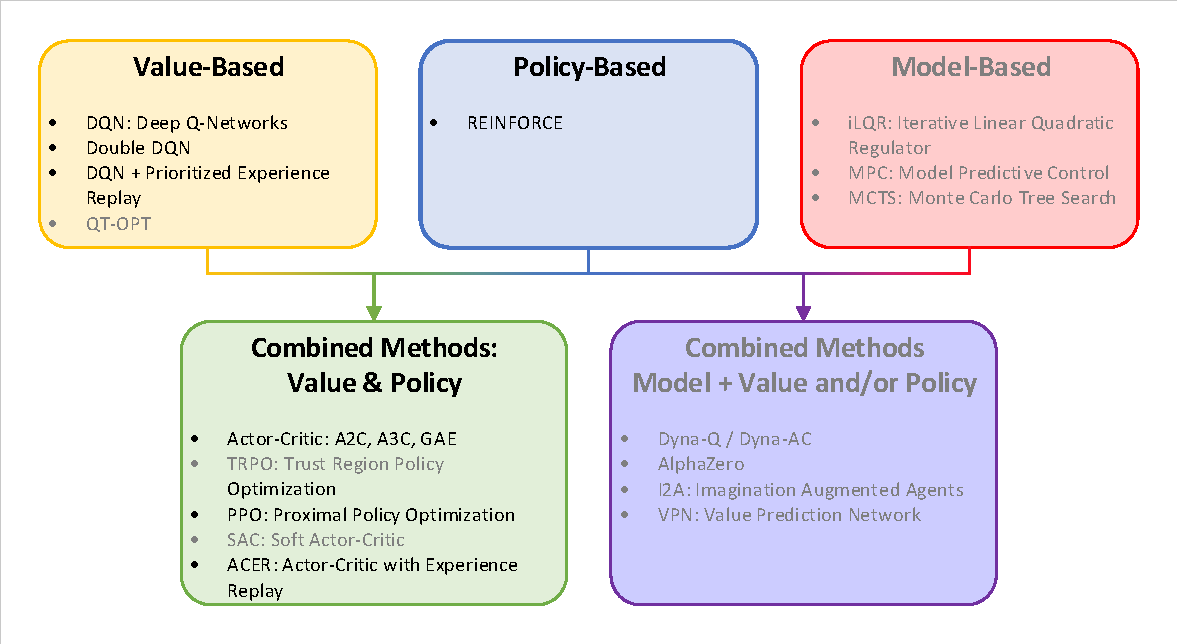
\includegraphics[clip, trim=10px 10px 10px 10px, width=0.95\columnwidth]{figures/rl/rl_families.pdf}
  \end{center}
  
  %\vspace*{-6pt}
  \caption[Overview of RL Families]{Overview of reinforcement learning families (adapted and extended from \cite{foundations2019graesser}). Methods that will not be used in this work are greyed out.}
  \label{fig:rl_families}
  %\vspace*{-12pt}
\end{figure}

In this work we will be focusing on actor-critic variants and value-based algorithms, so we will not cover model-based algorithms here. However we will be taking a look at policy-based methods, since they provide basic building blocks for the algorithms we will be using. \\ 
In this chapter we will begin with some basic ideas and challenges of reinforcement learning, as well as with some mathematical foundations in Section \ref{sec:concepts}. After that we will continue by introducing our first family of RL algorithms the value-based methods in Section \ref{sec:ValueMethods}. We will continue with a short overview over the idea of policy-based algorithms in Section \ref{sec:PGMethods} and will finally cover combined algorithms in Section \ref{sec:CombinedMethods} where we will focus on the actor-critic method and its successors.

\section{Key Concepts} \label{sec:concepts}
In this Section we give some basic insight into key concepts of reinforcement learning. First we give some basic intuition into how reinforcement learning works and what the challenges are when learning behavior from an unknown environment in Section \ref{ssec:rlidea}. We then continue by defining some of the basic terminology in Section \ref{ssec:rlterms} and finish with a different look on the RL problem from a mathematical point of view in Section \ref{ssec:RLMDP}.  

\subsection{Basic Ideas and Challenges} \label{ssec:rlidea}

Reinforcement learning at its core tries to solve some arbitrary decision-making problem. This problem is given by an \textit{environment} which produces information about its \textit{state} in form of an \textit{observation}. At each timestep an \textit{agent} receives the current observation and then acts according to some \textit{policy} by choosing from a set of available \textit{actions}. These actions should ultimately lead to the achievement of some objective inside of the environment. The behavior of the agent usually is encouraged by some kind of \textit{reward} which is returned by the environment. This basic agent-environment interaction loop is shown in Figure \ref{fig:rl_control_loop} \\ 

\begin{figure}[ht]
    
  \begin{center}
      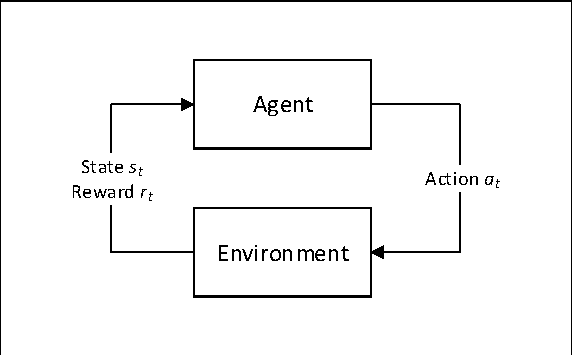
\includegraphics[clip, trim=10px 10px 10px 10px, width=0.6\columnwidth]{figures/rl/rl_control_loop.pdf}
  \end{center}
  
  %\vspace*{-6pt}
  \caption[Agent-environment interaction control loop]{The basic reinforcement learning control loop for agent-environment interaction.}
  \label{fig:rl_control_loop}
  %\vspace*{-12pt}
\end{figure}

This abstract setting can be used to solve a variety of tasks. We have three examples given in Figure \ref{fig:RLExamples}.
\begin{enumerate}
  \item \textbf{Playing the game Breakout.} Breakout is a game from the game console Atari. The goal of the game is to break the bars at the top, by reflecting a moving ball with a paddle at the bottom (like in Ping Pong). The observation is an rgb image of the game itself and the possible actions include resetting or firing the ball as well as moving the paddle to the left or right side of the screen. The reward is the current game score, which increments with every broken piece of barrier at the top. 
  \item \textbf{Playing the game of chess.} The input might be a complex representation of the positions of all pieces, or just a plain rgb-image. The possible actions change after every move, because they are dependent on the valid moves of all pieces. Reward might be as simple as winning ($+1$) or loosing ($-1$) the game, but can be more complex.
  \item \textbf{Grasping objects in a container.} A robotic arm should be trained to grasp arbitrary objects in a container. The observation is a plain image captured from above the robotic arm and a positive reward is given if the robot is able to successfully grasp an object. Actions include positioning the robot arm and opening or closing the "hand". 
\end{enumerate}

\begin{figure}[ht]
  \begin{center}
  \resizebox{0.95\columnwidth}{!}{%
  \begin{tabular}{ccc}
    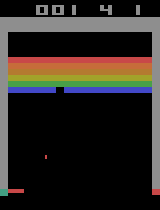
\includegraphics[clip, height=5cm]{figures/rl/Breakout.png}  &
  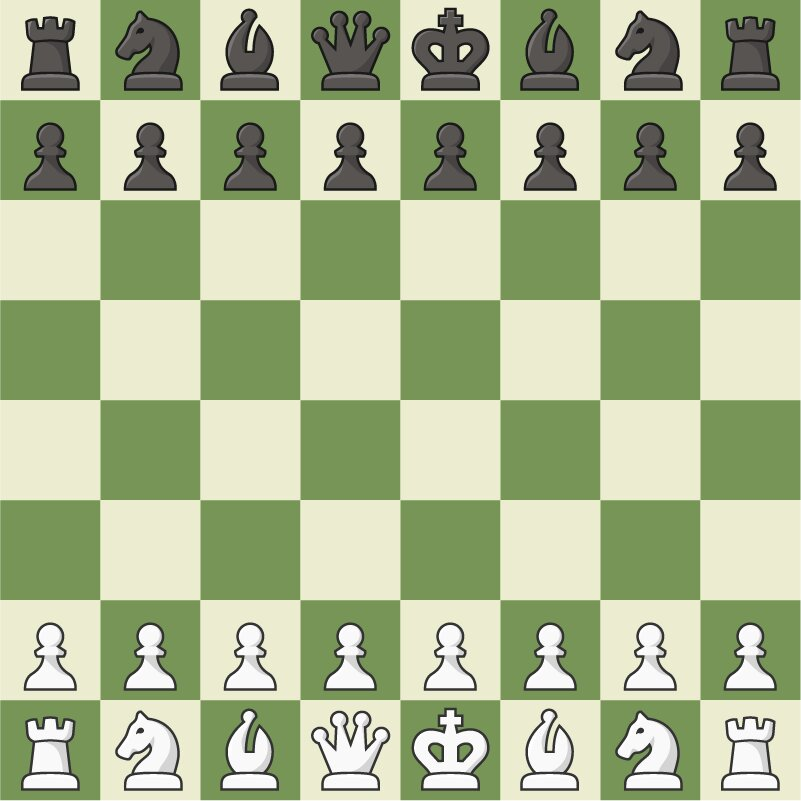
\includegraphics[height=5cm, keepaspectratio]{figures/rl/chess.jpg} & 
  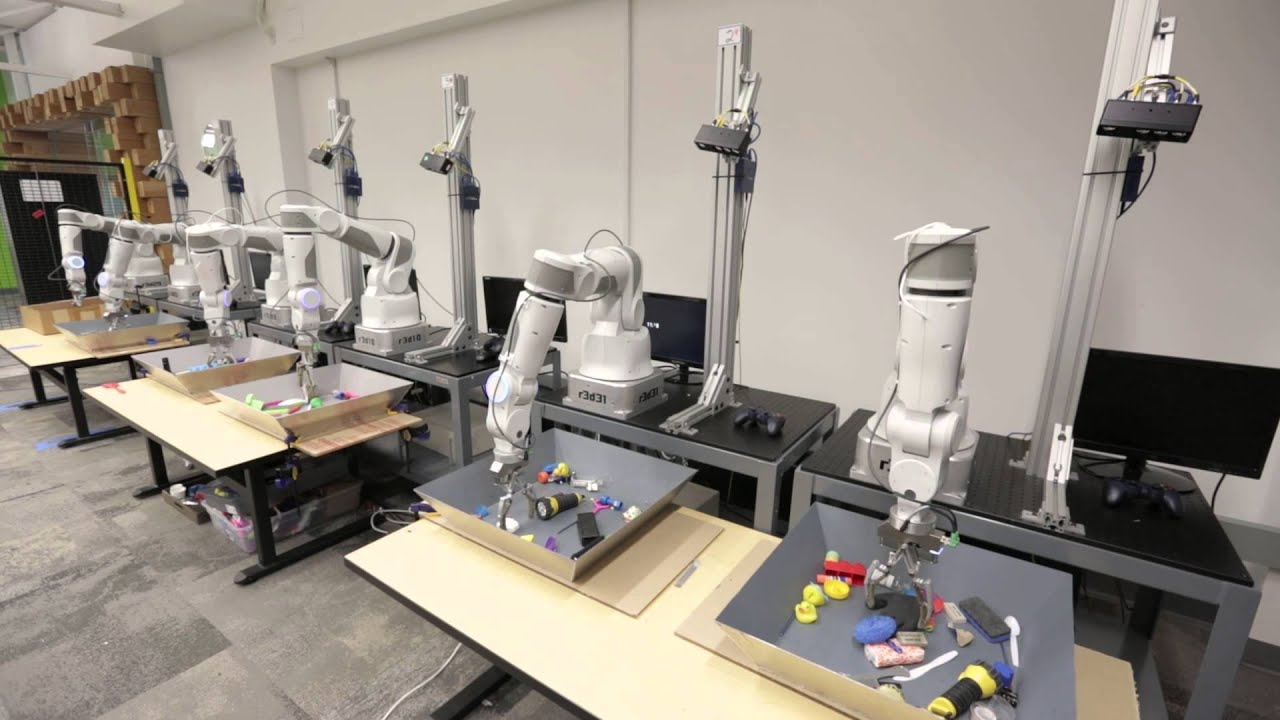
\includegraphics[trim=400px 0px 75px 0px, clip, height=5cm, keepaspectratio]{figures/rl/Google_Robot_Learning.jpg}\\
  {(a) The Atari game Breakout} &
  {(b) Chess\footnotemark} &
  {(c) Google Robot Grasping \footnotemark}\\
  
  \end{tabular}
  }%
  \end{center}
  %\vspace*{-12pt}
  \caption{Reinforcement learning examples.}
  \label{fig:RLExamples}
  %\vspace*{-12pt}
\end{figure}
  
\footnotetext{Image from chess.com \url{https://www.chess.com/bundles/web/images/offline-play/standardboard.6a504885.png}}
\footnotetext{Image from ai.googleblog.com \url{https://i.ytimg.com/vi/iaF43Ze1oeI/maxresdefault.jpg}}

Let's take a closer look at another example, pictured in Figure \ref{fig:CartPole}: The game of balancing a stick on a cart in a 2D environment. The sick can only be balanced by moving the cart, which has some velocity and can either be accelerated to the left or to the right. At each timestep the agent gets an observation which describes the current position and angle of the sick and can then choose which action it wants to take. If the stick falls over the agent looses. If it is able to balance the stick for more than 200 steps it wins. At each step it survives it gets a reward of $+1$. \\
Balancing a stick is harder than it initially seems to be. A simple algorithm which always moves the cart towards the direction the stick is leaning to, will always overshoot after a short time and loose balance. Of course we can think of a more complex algorithm and maybe solve the problem this way, but what if we want the computer to figure things out? How can we implement an algorithm which figures out on its own which actions should be taken for some given observation? How would we ourselves solve this problem? The answer is simple try and error. A human learns how to balance a stick, by balancing it. This will of course fail at the beginning, but after some time a human would get better and better at \textit{estimating} how the stick behaves in response to the actions that were taken. Similarly our reinforcement learning algorithm should just play around and looks at the results. Did the stick fell over? How long were we able to balance the stick? At which point did it fell and which actions led to that outcome? If we can answer all these questions we might be able to learn how to solve the problem. \\

\begin{figure}[ht]
  
  \begin{center}
      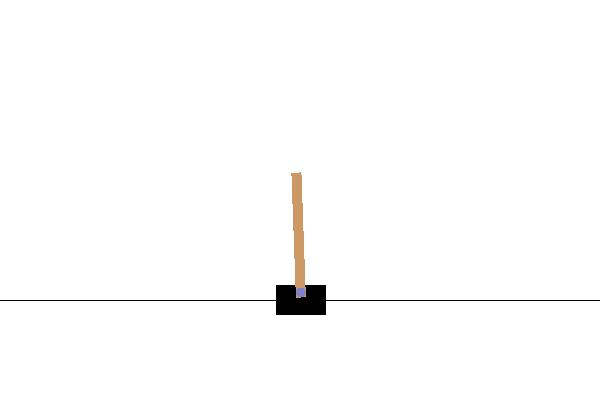
\includegraphics[trim=0px 50px 0px 100px, clip, width=0.6\columnwidth]{figures/rl/CartPole.jpg}
  \end{center}
  
  %\vspace*{-6pt}
  \caption[CartPole Environment]{A classic toy example from OpenAI gym \cite{openAIgym}: The CartPole environment.}
  \label{fig:CartPole}
  %\vspace*{-12pt}
\end{figure}


Building an association between some action and the resulting outcome in the environment is actually one of the greatest challenges for RL algorithms and known as the \textit{credit assignment problem}. Since rewards are typically sparse and delayed, understanding their origin is hard. Especially if you think about more complex games like chess, it is really unclear to what extend which move was responsible for winning or loosing a game. This problem becomes even greater the more sparse the rewards get: If we only reward winning or loosing, figuring out what made us win or loose is pretty hard, but if we reward or punish every single action, we might end up with a copy of an already known strategy. The challenge is to create an unbiased reward signal which does not distort the learning process. In the case of balancing a stick this is easy. Balancing the stick for a longer time is always good and can be rewarded. But as problems become more complex it is unclear if an action is actually good. If we take another look at chess for example, it might be beneficial to take a piece of your opponent, but it might also be better to go for a check or something which just gives you a positional advantage. Which action should be rewarded to what extend? In the end it is also a balance with how much time there is to learn. Sparse rewards will always result in longer training times, but give more freedom and thus might yield better results. \\
In the presence of sparse rewards another challenge arises: What if our learning algorithm is not able to find any solution at all? How can the algorithm know that there is a better solution out there, than the solution it already found? The answer is it cannot. The observations the agent makes in the environment are dependent on the taken actions. If the agent chooses the wrong actions it might never be able to explore the environment to a point where it receives more reward. The agent might get stuck with the false impression that it already achieved the maximum reward that is possible. \\
The last challenge we want to talk about is closely connected to the second one: Keeping the balance between exploration of the environment and exploitation of already learned behavior. Often diverging from already proven behavior decreases the short-term reward, but might lead to a much larger reward in the future. People face this problem in their everyday life: If you know the route from your home to some place, you are way more likely to take that route, than trying to find a shorter one, but risking the eventual failure. In this scenario the person - or in RL the agent - might get stuck in a situation where it never does anything else than taking the best known route, and get forever stuck in this local optimum.

\subsection{Terminology} \label{ssec:rlterms}
We already talked a lot about the existing challenges of reinforcement learning. Before we want to dive deeper into the various techniques that were developed to overcome these problems, we want to take a short look on the common terminology used throughout these algorithms.

\paragraph{States and Observations.}
For every environment there is a difference between the internal state $s$ of the environment and the observation $o$ an agent receives. While the state covers all information about the "world" the environment represents, the observation is a representation of that world and may or may not contain all information. Depending weather we can observe the whole environment or not, we talk about fully or partially observed environments. Observations are typically given to the agent as a real-valued vector. 

\paragraph{Actions.}
Actions are the things an agent can do in the environment. Most of the time they are fairly simple, like deciding to go left or right, but they can be more complex. \\
The set of actions an agent can perform in an environment is usually called the \textit{action space}. Depending on the environment, the action space might be discrete - with only a finite number of available choices - or continuous. Discrete action spaces are typical for game-like environment like CartPole or Breakout. Usually discrete actions are mutually exclusive, meaning only a single action can be chosen at a time: We can not go left and right - we have to choose. \\
Continuous action spaces on the other hand allow for a value attached to each available action and are often found in robot control tasks. For example if we look at a self-driving car, we have an action for the degree of the steering wheel and an action for the position of each pedal which need to be set in each step. \\
Not all RL algorithms are able to handle both types of action spaces. In some instances it is possible to transform continuous action spaces into discrete action spaces if no absolute precision is necessary. However this often results in a very high number of available actions.

\paragraph{Policies.}
Most of the time the words agent and policy will be used in the same manner. For the sake of clarity we want to define the policy as the rule(s) an agent uses to decide which action should be taken for some observation. We can think of the policy as the actors brain. \\
We denote the policy by $\mu$ if it is deterministic and $\pi$ if it is stochastic. Later when we are focusing on deep RL all of our policies will be build from artificial neural networks which are parameterized by their weights and biases. We therefore extend our notion to include these parameters as $\theta$ to have parameterizable policies $\mu_\theta$ and $\pi_\theta$. If the agent receives an observation at time $t$ it then generates the action according to its policy by:
\begin{align*}
  a_t &= \mu_\theta(o_t) \\
  a_t &\sim \pi_\theta(o_t)
\end{align*}


\paragraph{Episodes and Trajectories.}
We define an episode as a single run of an environment. So for chess an episode is a single game an agent played. While the agent played the episode it generates a \textit{trajectory} $\tau$, which is a sequence of triples from (state, action, reward), describing the episode:
\[\tau = ((s_0, a_0, r_0),  (s_1, a_1, r_1)) \]
The initial state of the environment is randomly sampled from some start-state distribution $\rho_0$. State transitions $s_t \rightarrow s_{t+1}$ happen according to the laws of the environment and the chosen action: $s_{t+1} = f(s_t, a_t)$. An episode might be infinitely long depending on the environment, which also leads to an infinite trajectory. In literature the words episode, trajectory and rollout are often used in a very similar fashion. 


\subsection{Reinforcement Learning as Markov Decision Process} \label{ssec:RLMDP}
In this section we want to take a look at the theoretical foundations of reinforcement learning. We will do this by looking at how we can model every RL problem with a discrete action space as a \textit{Markov Decision Process}. MDPs provide a mathematical framework for decision making processes and were introduced in the 1950s by Richard Bellman \cite{bellman1957markovian}. They were named after an earlier model the \textit{Markov Chains} which were created by the mathematician Andrey Markov who studied stochastic processes without memory. In this section we will see how MDPs build the foundations of value-based RL algorithms. \\
Before we talk about MDPs, let us take a step back and first talk about Markov Chains. In Markov Chains we have a fixed number of \textit{states} and \textit{transition probabilities} which define how likely it is to move from one state to another. We start in a given state and at each step the system randomly evolves from one state $s$ to another state $s'$. This transition only depends on the states' transition probability and is not related to earlier transitions. This is called the \textit{Markov Assumption}. Figure \ref{fig:MarkovChain} shows an example of a Markov Chain. \\

\begin{figure}[ht]
  
  \begin{center}
      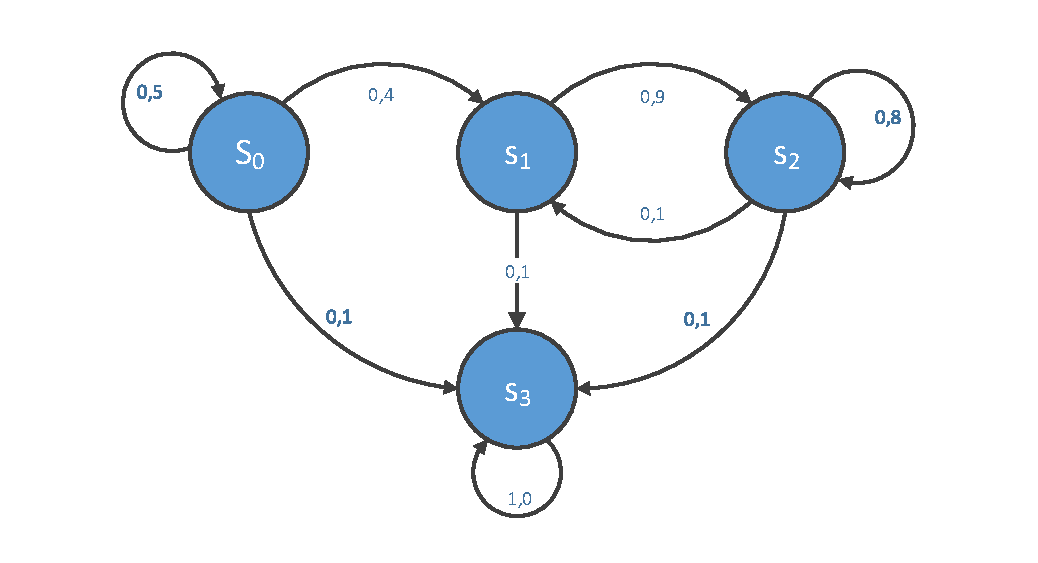
\includegraphics[trim=10px 10px 10px 10px, clip, width=0.8\columnwidth]{figures/rl/markov_chain.pdf}
  \end{center}
  
  %\vspace*{-6pt}
  \caption[An Markov Chain Example]{An example for a Markov chain. Suppose we start in $s_0$. There is a 50\% chance of staying in that state, a 40\% chance of transitioning to $s_1$ and a 10\% chance of transitioning to $s_3$. No matter how long it alternates between $s_0$, $s_1$ or $s_2$ at some point it will enter $s_3$ and remain there forever, because $s_3$ has a 100\% chance of transitioning to itself.}
  \label{fig:MarkovChain}
  %\vspace*{-12pt}
\end{figure}


Markov decision processes extend the idea of Markov chains with an active agent. At each step, the agent can choose from a set of actions and the state transition probability depends on the chosen action. Additionally each state transition may return some reward. The agents goal is to find a policy which maximizes the total reward over time. We extended our example from Figure \ref{fig:MarkovChain} with actions and rewards in Figure \ref{fig:MDP}. Like for Markov Chains, MDPs transition probabilities must only depend on the current state $s$ and the chosen action.\\

\begin{figure}[ht]
  
  \begin{center}
      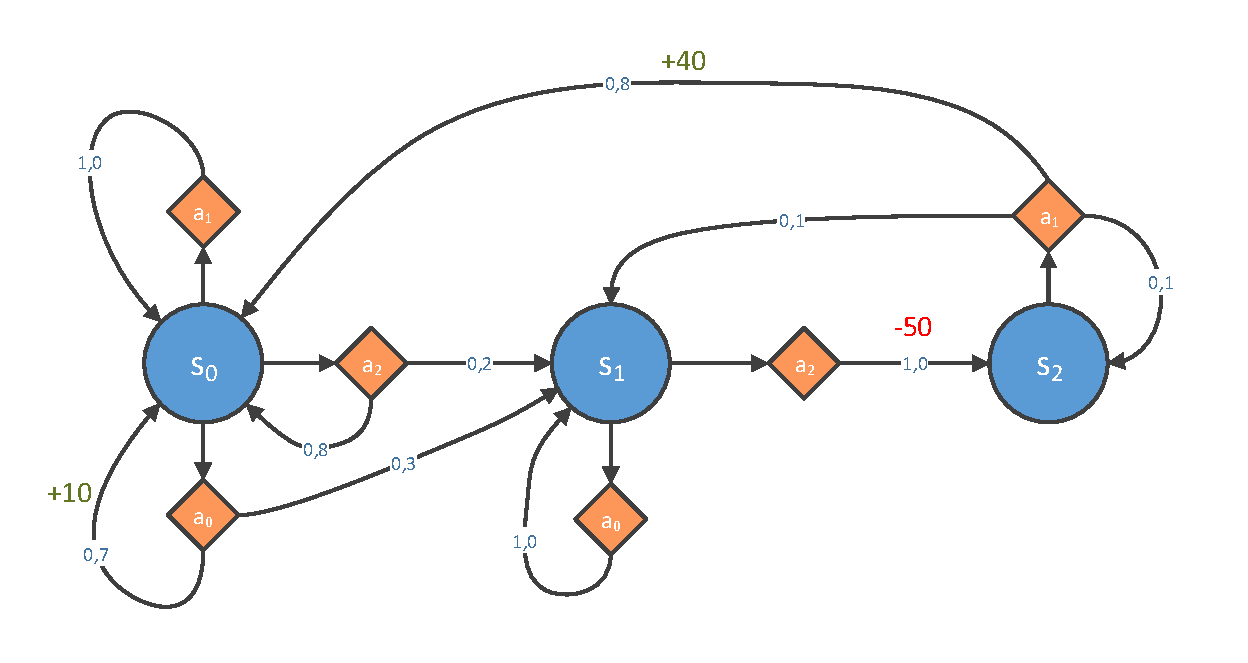
\includegraphics[trim=10px 10px 10px 10px, clip, width=0.9\columnwidth]{figures/rl/markov_decision_process.pdf}
  \end{center}
  
  %\vspace*{-6pt}
  \caption[An Example for the Markov Decision Process Example]{An example for the Markov decision process (recreated from \cite{handson2019geron}). Again we start in $s_0$ and the agent can choose from the actions $a_0$, $a_1$ or $a_2$. Choosing $a_0$ will give it a reward of $+10$. With a probability of 70\% the agent will be staying in $s_0$ and with a probability of 30\% it will transition to $s_1$. So the agent can likely repeat action $a_0$ in $s_0$ multiple times, but will at some point transition to $s_1$. In $s_1$ it now only has the options to stay there or go through a $-50$ penalty, which might even be repeated. The question is which strategy leads statistically to the most reward? Maybe choosing $a_0$ until we end up in $s_1$ and then never leave $s_1$ by always choosing $a_0$? Or going through the penalty and then collecting positive reward again? We will take a detailed look how we can solve this problem in the introduction of Section \ref{sec:ValueMethods}.}
  \label{fig:MDP}
  %\vspace*{-12pt}
\end{figure}

When modeling a RL problem as MDP we have a problem: The Markov assumption. If we look at the probability of our states, we would normally consider that at step $t$ the next state $s_{t+1}$ is sampled from a probability distribution depending on all the previous states and actions.

\[s_{t+1} \sim P\left(s_{t+1}|(s_0, a_0), (s_1, a_1), \dots, (s_t, a_t)\right)\]

 This sound logical, since the agent might also work with a stochastic policy which picks actions partially at random. Also reaching a state might influence other states or their transition probabilities. This not only violates the Markov assumption, it makes it extremely hard for an agent to approximate that underlying transition function for $P$ to make reasonable decisions in our environment. Therefore we need to simplify our model to:  

 \[s_{t+1} \sim P(s_{t+1}|(s_t, a_t)\]

This form sacrifices some freedom, but is still powerful enough and leads to much simpler transition functions which can be learned much easier. Despite the fact that a state transitions now only can depend on the last state and action, we can look at it from a different angle to reintroduce some of our freedom again. Any state can be defined to include any necessary information and there can be an unlimited (but fixed) number of states in our model. For example imagine a game where you if you win round one get a slight bonus for round two. Then the states and their transitions of round two would depend on round one. What we can do is introduce two completely new sets of states for round two where one set has the information attached that we won and one that we lost. This way the states for round two do not depend on round one, we just have more states and transitions. Using this trick helps us model many complex environments as MDP. \\
Agents in RL only decide upon an observation and not on the internal state of the environment. Also they normally do not know all states or their transition probabilities in the MDP. Therefore we often talk about a \textit{partially observable MDP} (\textit{POMDP}) in the context of reinforcement learning.

\paragraph{Reward and Return.} %TODO: Image/Example for discounted reward.
in our model, the agent may receive some reward after or during each state transition: $r_t = R(s_t, a_t, s_{t+1})$. The agents goal is to maximize the total sum of expected reward, but - as we discussed earlier - it is complicated to know which action action was responsible for which reward. If we look back at the example from Figure \ref{fig:MDP}: How much reward do we generate by choosing $a_0$ in $s_0$? We have a probability of generating $+10$ reward, but we might also get no reward and end up in $s_1$. How much reward we are able to generate once we ended up in $s_1$ is also unclear. \\
To build a better connection between actions and reward, instead of associating rewards directly with the action which was chosen right before the reward was returned, we calculate the return $R$. The return is defined as a sum of future rewards, which we are able to achieve from the current state when choosing a certain action. Depending on the task, this sum can be formulated in different ways. This way an action which results in negative reward can actually be actually seen as a good action, if it generates much more positive reward in the future and the other way around.  \\
Since most of the time, the current action is not directly associated with every future reward, we look at so-called \textit{discounted rewards}. We call this reward the \textit{finite-horizon discounted return} with a discount factor $\gamma \in [0, 1]$:

\[R(\tau) = \sum_{t=0}^T \gamma^t r_t\]

The discount factor is an important variable which controls how much we value future rewards and needs individual tuning for every environment. Small values for $\gamma$ lead to more "shortsighted" actions - with the extreme case $\gamma = 0$ valuing just the initial (next) reward. The other extreme case with $\gamma = 1$ just means there is no discount and which therefore is called the \textit{finite-horizon undiscounted return}: 
\[R(\tau) = \sum_{t=0}^T r_t\] 

Sometimes we are also dealing with environments with infinite episode lengths. If $T$ is unbounded we talk about an \textit{infinite-horizon discounted return}. In this case $\gamma$ needs to be smaller than 1 to bound our future rewards.

\paragraph{The RL Problem.}
Before we look at the first RL algorithm, we want to give a mathematical definition for the reinforcement learning problem itself. If the goal of the agent is to maximize the total reward from the environment, RL algorithms will select a policy which at each step maximizes the \textit{expected return} by choosing an optimal action $a^*$ under observation $o$. Depending on the chosen discount factor this return will depend more or less on future rewards. \\ 
Lets look at an example, where both the environment transitions and the policy are stochastic. The probability for a trajectory with $T$ steps is: 

\[P(\tau|\pi)=\rho(s_0)\prod_{t=0}^{T-1}P(s_{t+1}|s_t, a_t)\pi(a_t|o_t)\]

We denote the \textit{expected return} for the current policy $\pi$ by $J(\pi)$. For some trajectory $\tau$ this return is equal to:

\[J(\pi) = \int_\tau P(\tau|\pi)R(\tau) = E_{\tau\sim\pi}\left[R(\tau) \right]\]

In case of finite-horizon discounted return we get 

\[J(\pi) =  E_{\tau\sim\pi}\left[R(\tau) \right] = E_\tau\left[\sum_{t=0}^T \gamma^t r_t\right]\]

Given this definition for expected return, we can formulate the problem of reinforcement learning as the problem of computing an optimal policy $\pi^*$ which maximizes expected return over a trajectory:
\[\pi^*=\argmax_\pi J(\pi)\]

\section{Value-Based Methods} \label{sec:ValueMethods}
In this section we want to take a look at the first family of reinforcement learning algorithms: The value based methods. We begin by looking at a technique called \textit{value iteration}, which will allow us to calculate state values in a MDP, in Section \ref{ssec:Value_Iteration}. We will then continue to explore how this technique can be used to learn state-action values (called $Q$-values) from a partially unknown MDP in Section \ref{ssec:TDLearning}, which leads directly to our basic value-based RL algorithms \textit{SARSA} (Section \ref{ssec:SARSA}) and the \textit{Q-Learning algorithm} (Section \ref{ssec:Q_Learning}). Finally we will combine the Q-Learning algorithm with neural networks into Deep Q-Learning in Section \ref{ssec:DeepQLearning} and look at a number of Deep Q-Learning extensions in Section \ref{ssec:DQNExtensions}. 

\subsection{Value Iteration} \label{ssec:Value_Iteration}

In Section \ref{sec:concepts} we already saw that we can express our RL problem as a Markov decision process. Bellman did not only create the model, but also found a way to estimate the optimal state value of any state in an MDP. This state value is calculated by looking at all discounted future rewards an agent can expect if it currently is in state $s$ and then acts optimally for all future transitions. In the Equation \ref{eq:Optimal_State_Value} $T(s, a, s')$ denotes the transition probability for state $s'$ if the agent is in state $s$ and chooses action $a$.  

\begin{equation} \label{eq:Optimal_State_Value}
V^*(s) = \max_a \sum_{s'} T(s, a, s')\left[ R(s, a, s') + \gamma V^*(s')\right]
\end{equation}

We can see that the equation is recursive, since we calculate the value for the current state by adding the transition reward to the state values of the possible next states weighted by their transition probability. We also discount the value of the next state by our discount factor $\gamma$. Bellman described a simple a algorithm called \textit{value iteration} which calculates this optimal state value \cite{bellman1957markovian}. It works by initializing all state values to zero and iteratively calculating

\[V_{k+1}(s) = \max_a \sum_{s'} T(s, a, s')\left[ R(s, a, s') + \gamma V_k(s')\right]\]

Fortunately this algorithm is guaranteed to converge. Depending on how interested we are in exact values, we can always cancel the iteration early and look at the intermediate results in the $k$th iteration. The problem is knowing the current value of the state we are in does not tell us which action we should take next. The equation is not suited to derive a policy from it. Luckily Bellman also found, that it is easy to reformulate the equation to calculate $Q^*(s, a)$ which is the optimal value we can expect if we choose action $a$ and then always act optimally. We define this value in Equation \ref{eq:Optimal_Q_Value}. This value can again be calculated by value iteration, as can be seen in Equation \ref{eq:Q_Value_Iteration}:

\begin{align}
  Q^*(s, a) &= \sum_{s'} T(s, a, s')\left[ R(s, a, s') + \gamma \max_{a'} Q^*(s', a')\right] \label{eq:Optimal_Q_Value}\\
  Q_{k+1}(s, a) &= \sum_{s'} T(s, a, s')\left[ R(s, a, s') + \gamma \max_{a'} Q_k(s', a')\right] \label{eq:Q_Value_Iteration}
\end{align}

With the optimal Q-value at hand, defining the optimal policy is as easy as defining $\pi^*(s) = \argmax_a Q^*(s, a)$. So are we at the end? Do we have the ultimate tool for every RL problem? Sadly the answer is no, because while we could calculate our policy exactly in that way, we do not have the information to do so. In a real RL scenario we do not know the underlying MDP - we have to discover all states, rewards and transition probabilities first. 

\subsection{Temporal Difference Learning} \label{ssec:TDLearning}
The basic algorithm used for Q-Learning is called \textit{Temporal Difference Learning} (TD Learning). This algorithm is very similar to the value iteration method and also connected to the stochastic gradient decent algorithm. The unknown MDP is usually explored using a stochastic policy. In the easiest case this policy is just sampling a random action from our action space for each state. We then iteratively improve our state estimation by calculating:

\[V_{k+1}(s) \leftarrow (1-\alpha) V_k(s) + \alpha (r + \gamma V_k(s')) \]

In this equation $\alpha$ is a parameter for the learning rate in the interval $[0, 1]$. The term is usually rewritten to emphasize that we change our estimation by having an error term:

\begin{equation*}
  V_{k+1}(s) \leftarrow V_k(s) + \alpha \underbrace{(\underbrace{r + \gamma V_k(s')}_\text{TD Target} - V_k(s))}_\text{TD Error}
\end{equation*}

Again the basic TD learning method is formulated for the value function and we have to reformulate it for Q-Value estimation. Also we now have to decide how we explore the environment. Depending on our choices we end up with either \textit{SARSA} or the classical \textit{Q-Learning} algorithm.

\subsection{SARSA} \label{ssec:SARSA}
We are finally at the point where we can look at the first reinforcement learning algorithm: SARSA, which was proposed by Rummery and Niranjan in 1994 \cite{rummery1994line}. SARSA uses the same method or values to sample actions and learn from them, therefore SARSA is a so called \textit{on-policy} learning algorithm. We will talk about the difference to \textit{off-policy} algorithms in a moment when we come to classical Q-learning. \\ 
The name SARSA was not originally proposed, but is widely used and comes from the parameters that are needed to make a single update step. The agent which currently is in state $s$ takes action $a$ and gets return $r$. It then samples a new action based on $s'$ from its policy (which is a stochastic policy) and chooses action $a'$, combined we get  state-action-reward-state-action $(s, a, r, s', a')$ - the origin of the name. \\

SARSA uses the TD-learning method to update its Q-value estimation:

\[Q_{t+1}(s, a) \leftarrow Q_t(s, a) + \alpha (r + \gamma Q(s', a') - Q(s, a))\]

For each state-action pair, SARSA calculates a running average of the rewards $r$ combined with the sum of expected discounted future reward. This way SARSA is able to estimate optimal Q-values for every state-action pair given enough iterations. We included a sketch of this procedure in Algorithm \ref{alg:SARSA}.

\begin{algorithm}[ht]
  %\KwData{}
  \KwResult{Estimated Q-Values for $Q(s, a)$}
  Initialize $Q(s, a)$ for $\forall s \in S$ and $\forall a \in A$ randomly. $Q(terminal, \cdot) = 0$ \;
 \ForEach{episode}  {
   $s \sim \rho(\cdot)$ \tcp*[f]{Sample initial state}\;
   Choose $a$ from $s$ using a policy derived from $Q$ (e.g. $\epsilon$-greedy) \;
   
   \ForEach{step in episode}  {
     Take action $a$, observe $r$, $s'$ \;
     Choose $a'$ from $s'$ using policy derived from $Q$ (e.g. $\epsilon$-greedy) \;
     $Q(s, a) \leftarrow Q(s, a) + \alpha (r + \gamma Q(s', a') - Q(s, a))$ \;
     $s \leftarrow s'$, $a \leftarrow a'$ \;
   }
 }
  \caption[The SARSA Algorithm]{SARSA Algorithm for On-Policy TD Q-Value Estimation (adapted from \cite{sutton2018reinforcement})}\label{alg:SARSA}
 \end{algorithm}

We just mentioned that actions are sampled from our policy, but what exactly is our policy? To this point we only talked about the calculation of Q-values. If we already calculated all our Q-values, it seems to be clear that the best policy would be to always choose the action for the current state with the highest Q-value. The problem when learning is we do not know the best Q-value for each state yet. At this point we come back to a problem we discussed in Section \ref{ssec:rlidea}: The balance between exploration and exploitation. We need a policy which explores the environment in a way that allows us to calculate Q-values for every state. Therefore we need a policy which will visit each state - not only once multiple times to get sufficient good Q-Value estimations. \\ 
If we strictly follow an exploration policy which already exploits our estimated Q-values we will likely end up only exploring a fraction of all states and get stuck in a local optimum. So instead we will use a stochastic policy in SARSA. If we take the other extreme and use a completely random policy the agent will always be able to visit all states eventually, but may need extremely long to do so. Therefore the most commonly used policy is an $\epsilon$-greedy policy, which combines a stochastic exploration with an estimated Q-Value exploitation. In this policy at each step we have the probability $\epsilon$ for which we take a random action and with probability $(1 - \epsilon)$ we choose the action with the highest Q-value. This way we will explore the environment enough, but still direct learning to be more focused on promising states. Often times $\epsilon$ will not be set to a fixed value. Instead $\epsilon$ will be a function over the course of the training process, starting with high values (mostly random actions) and then gradually decreasing over time. 

\subsection{Q-Learning} \label{ssec:Q_Learning}
Q-Learning actually predates SARSA, and was developed in 1992 by Chris Watkins \cite{watkins1992q}. Today, Q-Learning is one of the most popular methods in RL. As for SARSA, in Q-Learning we estimate state-action values with the TD learning algorithm. The difference is that we are now dealing with an off-policy algorithm. This means that the policy that is being trained is not (or only partially) executed during the training process. You can find the procedure in Algorithm \ref{alg:QLearning}.  

\begin{algorithm}[ht]
  %\KwData{}
  \KwResult{Estimated Q-Values for $Q(s, a)$}
  Initialize $Q(s, a)$ for $\forall s \in S$ and $\forall a \in A$ randomly. $Q(terminal, \cdot) = 0$ \;
 \ForEach{episode}  {
   $s \sim \rho(\cdot)$ \tcp*[f]{Sample initial state}\;
   \ForEach{step in episode}  {
    Choose $a$ from $s$ using exploration policy (e.g. random or $\epsilon$-greedy) \;
     Take action $a$, observe $r$, $s'$ \;
     $Q(s, a) \leftarrow Q(s, a) + \alpha (r + \gamma\max_{a'} Q(s', a') - Q(s, a))$ \;
     $s \leftarrow s'$\;
   }
 }
  \caption[The Q-Learning Algorithm]{Basic Q-Learning Algorithm for Off-Policy TD Q-Value Estimation (adapted from \cite{sutton2018reinforcement})}\label{alg:QLearning}
 \end{algorithm}

We can see that while both algorithms are pretty similar, there are a few differences. Instead of using a stochastic policy and using that policy to choose an action $a$ \textbf{and} for estimating the future reward (the $Q$ value), we now only use a stochastic policy to sample $a$ and then always use a greedy policy. This can be interpreted in a way that the algorithm considers its estimated Q-Values to be optimal even if they are not. Therefore our update rule becomes: 
\[Q_{t+1}(s, a) \leftarrow Q_t(s, a) + \alpha (r + \gamma\max_{a'} Q_t(s', a') - Q_t(s, a))\]

Q-Learning even works if the exploration policy is completely random, even though $\epsilon$-greedy type strategies are often faster. So again, are we finished yet? If Q-Learning is able to calculate optimal Q-Values and thus provides us with an optimal policy we can now always use Q-Learning, right? The problem is while Q-Learning is able to calculate the optimal Q-values, it may need a very long time to do so. And since Q-Learning uses a table for every state that is possible in our environment, problem size exponentially increases for many environments. \\
If you think of the simple game of Tic-Tac-Toe we have 9 boxes where each player may set his mark, so end up with $2*2^9+9=1033$ possible states. For such a simple game thats a surprisingly high number. And it gets even worse if we look at games which allow for even more combinations. If we take the computer game classic \textit{Pac-Man}, we can see every coin the player can capture as a single state. With around 100 coins we are already at $2^{100} \approx 10^{30}$ states. And the coins are not the only thing which may change state in that game. With traditional Q-Learning we would not only need ages to explore all states, we would also end up with a huge table of state-action values which might not fit in our memory. \\

\subsection{Deep Q-Learning} \label{ssec:DeepQLearning}
When we are dealing with a huge number of states, we might want to sacrifice some of the accuracy of our predictions for the sake of actually being able to compute these predictions in a reasonable time. To achieve this instead of computing a table containing a value approximation for every state-action pair we will compute a (nonlinear) function which approximates these values. Ideally this function should have an amount of parameters which is much smaller than the number of possible states. We denote this function as $Q_\theta(s, a)$. As we know from Chapter TODO artificial neural networks are highly nonlinear parameterizable functions. This means we can use neural networks to approximate our Q-values. In 2013, the DeepMind team showed, that using deep neural networks for Q-value approximation has a stellar performance on playing multiple games from the Atari 2600 game console \cite{mnih2013playing}. Their work also proved, that it is not necessary to handcraft features for the neural network. Instead a raw image from the game is sufficient and even results in better performance. \\
We call a deep neural network that is used for Q-Value estimation a \textit{Deep Q-Network} (DQN) and indicate that our Q-value is estimated by subscripting our Q-function with $\theta$ denoting the parameters of our neural network. Using a DQN for approximate Q-Learning is called \textit{Deep Q-Learning}. \\
To train a neural network we still need a key element: A loss function. The loss function should represent how much the value calculated by the neural network deviates from the target value. Similar to how we calculated our updates in classical Q-Learning we treat our estimation as if we already know the best Q-Values. Our target Q-Value then is 

\[Q_{target}(s, a) = r + \gamma \cdot \max_{a'}Q_\theta(s', a')\]

Using a common metric like the mean square error we can calculate the difference between the estimated Q-Value of our network and the target Q-Value to get a loss function.

\[\mathcal{L} = (Q(s, a) - Q_{target}(s, a))^2\]

\begin{figure}[t]
  
  \begin{center}
      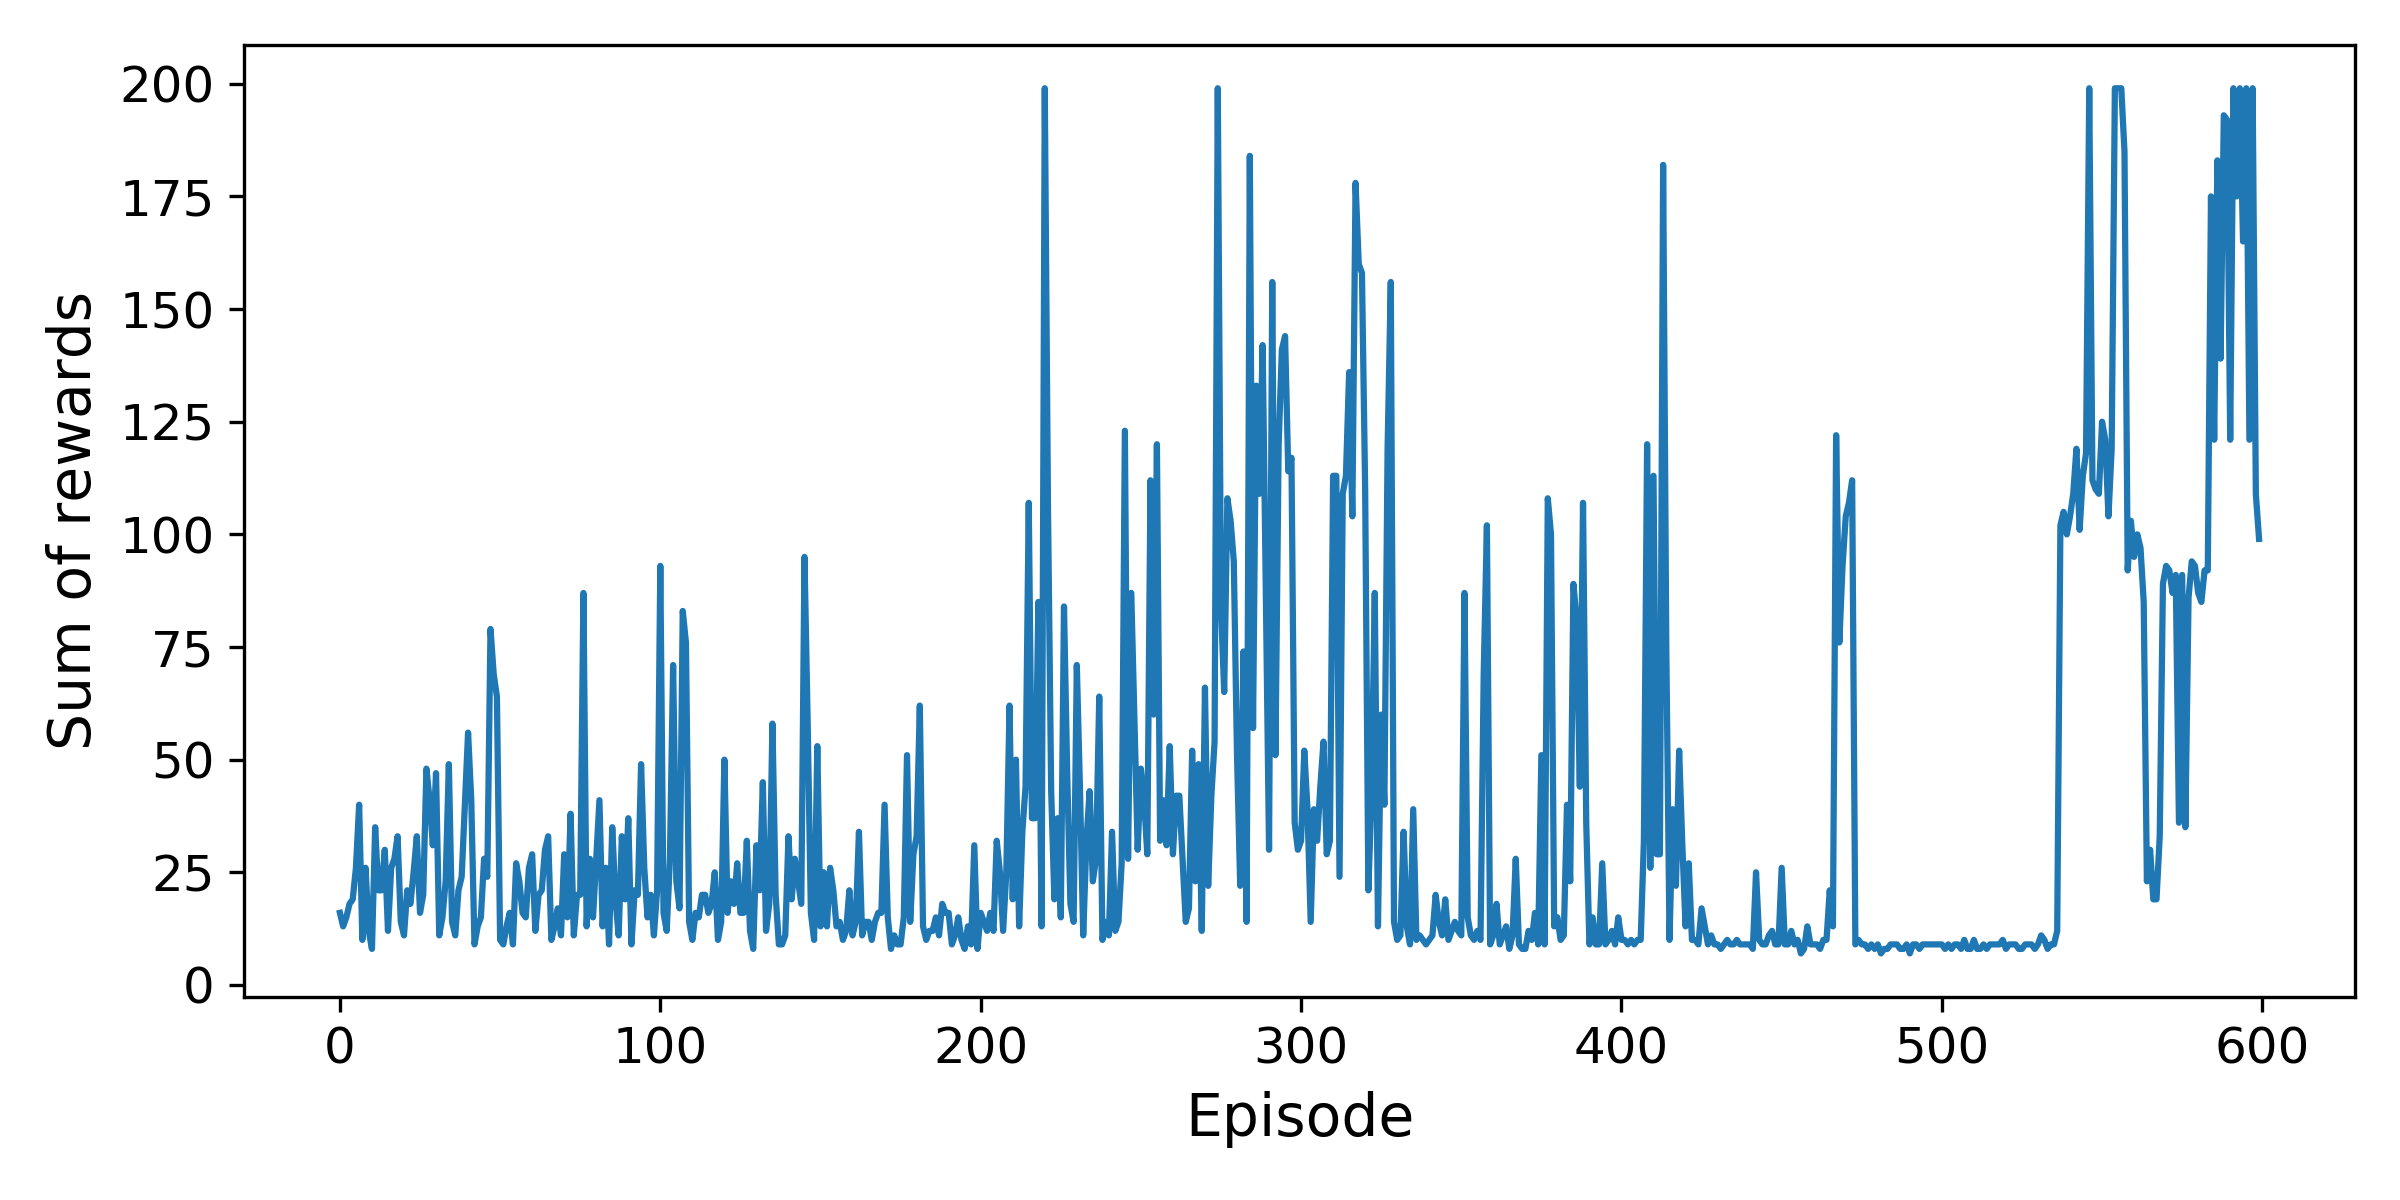
\includegraphics[clip, width=0.8\columnwidth]{figures/rl/dqn_cart_pole_plot.png}
  \end{center}
  
  %\vspace*{-6pt}
  \caption[Learning Curve for Deep Q-Learning on CartPole]{Learning Curve for basic Deep Q-Learning only with simple experience replay on the CartPole environment.}
  \label{fig:learning_curve_dqn}
  %\vspace*{-12pt}
\end{figure}

By defining a loss function we can train our neural network in the same fashion as in supervised learning using the well-known stochastic gradient decent algorithm. This will need thousands or even millions of updates to converge - if it ever does. Deep Q-Learning in its basic form suffers from a lot of problems which results in a DQN learning either slowly, not at all, or suffering from a problem called \textit{catastrophic forgetting}. Figure \ref{fig:learning_curve_dqn} shows the reward over time when solving the CartPole environment. As we can see the agent does not learn anything for 300 episodes, then suddenly achieves the maximum possible reward of 200 and then seems to forget what it has learned. This process then alternates back and forth. Problems like this emerge from a number of different problems:
 \begin{enumerate}
  \item The SGD algorithm assumes that we have data that is \textit{independent and identically distributed} (i.i.d), but our training data is neither independent nor identically distributed. Our samples are generated in episodes which typically make state transitions between states which have a lot in common (e.g. two adjacent frames in a game). Also the distribution of our data is not similar to the distribution the data would have if it has been sampled from an optimal policy. 
  \item We learn from data generated by our current policy (or from a partially random policy in case of $\epsilon$-greedy), which will create samples which are highly correlated. Additionally we use the same model we created our samples with to set our target value and calculate our loss. This may result in a feedback loop which makes training unstable.
  \item In training, the agent will likely overestimate Q-Values. This is due to the nature of the update process. In each step, the target model will select the highest Q-Value, but all Q-Values are estimated. Think of a situation in which each action for a given state has the same Q-Value. An approximation will never be exact, so some of the Q-Values will be slightly higher and some will be slightly lower. When selecting the next Q-Value we do not go for an average we select the highest. Thus we are always prone to overestimation.
 \end{enumerate}

 All these problems combined lead to a very unstable learning process. Fortunately over the years many extensions were developed to reduce their impact dramatically.

\subsection{DQN Extensions} \label{ssec:DQNExtensions}
In this section we want to give a brief overview over techniques that were developed to make Deep Q-Learning more stable. 

\paragraph{Experience Replay.}
At first we want to focus on breaking the correlation between the samples. If we always train from a single episode all our training data will be highly correlated and states will look almost identical. To overcome this instead of learning directly from the trajectory generated by a single episode we introduce a \textit{replay buffer}. After playing an episode we draw random samples from our buffer and learn from them. This will break up the correlation between samples and also reduces the danger of forgetting already learned behavior. On the negative side it introduces new hyperparameters with the size of the replay buffer and the number of samples we want to draw for learning, which are both dependent on the task we are trying to solve. 

\paragraph{Prioritized Experience Replay.}
Lets take the idea of the replay buffer to the next level: Since not all of our samples might be equally important for the learning process, it would be a good idea to replay interesting samples more often than others. This procedure is called \textit{importance sampling} (IS) or \textit{prioritized experience replay} (PIR) and was developed in 2015 by the DeepMind Team \cite{schaul2015prioritized}. The question is what are interesting samples? Schaul et al. proposed to use the TD error term $\delta = r+\gamma V_k(s') - V_k(s)$ (see Section \ref{ssec:TDLearning}) as an indication of a sample being interesting. This makes sense if you think about what a large error means for our algorithm: If we estimated a state value wrong, it is equal to saying we are surprised by the result of the state value. Thus the sample is interesting. \\
In our replay buffer we now assign a priority to each sample, depending on how large the TD error is. We set this priority to a high value for the first time, to ensure that the sample will be sampled at least one time and update the sample priority each time it is sampled to $p = |\delta| + \epsilon$ with $\epsilon$ being a small positive constant to ensure each sample has a non-zero probability of being drawn. A single sample then has the probability of 

\[P(i) = \frac{p_i^\alpha}{\sum_k p_k^\alpha}\]

The exponent $\alpha \in [0, 1]$ is a new hyperparameter which defines how much weight is given to importance sampling with $\alpha = 0$ being standard uniform experience replay.  \\
With some samples being sampled more often than others we again violate our goal of learning uniformly on samples from the target distribution that would be observed if the agent would behave optimally. Without a compensation for this bias, our agent would overfit on those high priority samples. To compensate, we downweight more important samples in training by 

\[w_i = \left(\frac{1}{N} \cdot \frac{1}{P(i)}\right)^\beta\]

where $\beta \in [0, 1]$ is another hyperparameter which controls how much we want to compensate (0 means no compensation). PIR has shown to vastly improve convergence speed and overall performance of Deep Q-Learning, but also introduces two additional hyperparameters which need to be tuned.

\paragraph{Target Networks.}
The next extension aims at improving training stability and reducing the problem of a feedback loop. Since we use the same network to generate samples and to calculate the target Q-Values, situations where training is unstable, diverges or oscillates are very likely. This can be broken up by separating the prediction when generating samples from the calculation of the target values. This is done by working on two similar - but not identical - copies of the same network. We call one of them the \textit{online model} and one the \textit{target model}. The online model will interact with the environment and get updated in the regular update step, while the target model only makes the predictions for the target Q-Value. Every once in a while we copy the weights of the online model to the target model.

\paragraph{Double DQN.}
Next up we want to reduce Q-Value overestimation. This can be done by improving the usage of our target network: Instead of always selecting the action with the highest Q-Value for the Q-target in the update step, we select the action with the highest Q-Value from the online model, and then use the Q-Value estimation for that action from the target DQN. This method was also developed by DeepMind and is called \textit{Double DQN} (DDQN) \cite{van2016deep}.

\paragraph{Dueling DQN.}
Another technique which aims at stabilizing learning is called Duelling DQN \cite{wang2015dueling} (not to be confused with Double DQN). Duelling DQN changes the architecture of the DQN to not compute Q-Values directly, but rather compute two values: The state value $V(s)$ and the so-called \textit{advantage} $A(s, a)$. The advantage expresses how good it is to take an action $a$ in state $s$ in comparison with every other action. If we look at the advantage for an optimal policy $A^*(s, a)$, the best action $a^*$ will have an advantage of 0. We can express the Q-Value as $Q(s, a) = V(s) + A(s, a)$. Computing multiple values which are connected to the same task proves to be beneficial for the training of neural networks and greatly stabilizes training. Therefore we extend our neural network to compute both $V(s)$ and $A(s, a)$ for every action.  %TODO: Source? 

\paragraph{Even more extensions.}
We already discussed a lot of important extensions for Deep Q-Learning, but there are even more. Update steps can be combined into multi-step learning which further stabilizes the training process \cite{sutton1988learning}. Instead of learning to approximate the returns we can also learn to approximate the distribution of returns \cite{bellemare2017distributional}. Like for every neural network the introduction of noise often results in more robust predictions. Additionally the introduction of noise is beneficial in RL because it improves exploration \cite{fortunato2017noisy, plappert2017parameter}. \\

Most of the techniques to improve Deep Q-Learning that were discussed can also be used in conjunction. In 2018 the DeepMind team created an agent which they called \textit{Rainbow} and which was able to outperform all standalone techniques on the Atari 2600 benchmark \cite{hessel2018rainbow}. Even though this proves that the combination of these extensions can be beneficial, the introduction of several new hyperparameters requires careful fine-tuning which might take a lot of time even with modern hyperparametersearch algorithms. %TODO: Make figure for learning with extensions.

\section{Policy Gradient Methods} \label{sec:PGMethods}
We already saw, that Q-Learning (with its extensions) is a very powerful tool to solve RL problems. Nevertheless we also saw that Q-Learning suffers from a lot of problems and with all its extensions is hard to parameterize correctly. Also we are not able to solve RL problems with continuous action spaces, since there would be an infinite number of actions to choose from. Therefore we need an alternative way to deal with reinforcement learning problems. \\
Let us look at what we are doing in Q-Learning: We estimate values $Q_\theta(s, a)$ and then derive an optimal policy by $\pi^*(s) \approx \argmax_a Q_\theta(s, a)$. So we are only indirectly learning an optimal policy. While the Q-Value might be interesting, at the end we do not need to know how much better an action is compared to others. We are only interested in acting optimally. So instead of estimating Q-Values and then deriving an optimal policy, we want to directly learn the optimal policy. This is the idea behind \textit{Policy Gradient} (PG) methods which aim at iteratively computing an optimal policy by using gradients in policy space. \\
We will only look into a single member of this family in Section \ref{ssec:REINFORCE}: The REINFORCE algorithm. This is because the PG-methods quickly involved into combined methods which take ideas from both Q-Learning and REINFORCE and combine them to achieve even better results.

\subsection{REINFORCE} \label{ssec:REINFORCE}
The REINFORCE algorithm was invented in 1992 by Ronald Williams \cite{williams1992simple}. The algorithm computes a policy which produces action probabilities directly from states. Like in Deep Q-Learning we use a neural network as our policy, which directly outputs probabilities for actions in the discrete case and values for actions in a continuous setting. The name REINFORCE originates from the simple idea of positively reinforcing actions which proved to yield good results while discouraging actions which yield bad results. This reinforcement is done iteratively in small steps by application of policy gradients.

So let us begin by defining what a policy gradient should be. Remember our definition for expected return $J(\pi)$ from Section \ref{ssec:RLMDP}. We extend our notion to also include the parameters of our neural network. We can then define our goal as finding the parameters for our network which maximize the expected return:  

\begin{equation} \label{eq:PGObjective}
  \max_\theta J(\pi_\theta) =  E_{\tau\sim\pi_\theta}\left[R(\tau) \right]
\end{equation}

So how do we maximize the expected return and find the correct parameters? If we look at our objective $J(\pi_\theta)$ we can think of it as an abstract hypersurface for which we are trying to find a maximum. The dimensions of the surface are given by the network parameters $\theta$ and the "height" is our return. To gradually improve our policy, we are using gradient ascent (which is the same as gradient descent, but now we are using the gradients to find a maximum) for $J(\pi_\theta)$

\[\theta \leftarrow \theta + \alpha \nabla_\theta J(\pi_\theta)\]

The gradient $\nabla_\theta J(\pi_\theta)$ is our \textit{policy gradient} and $\alpha$ is our learning rate. But at this point we have a problem: If we look at Equation \ref{eq:PGObjective} we can see, that $\nabla_\theta J(\pi_\theta)$ is not differentiable with respect to $\theta$ because $R(\tau)$ is not dependent on $\theta$. Also the function $R(\tau)$ itself is unknown. Since the expected reward is directly dependent on the decisions of the current policy, it is possible to rewrite the equation into a form that is differentiable:

\begin{equation} \label{eq:PGEstimation}
  \nabla_\theta J(\pi_\theta) = E_{\tau \sim \pi_\theta} \left[\sum^T_{t=0}R_t(\tau) \nabla_\theta \log \pi_\theta(a_t|s_t)\right]
\end{equation}

We omit the proof here, but it can be found in \cite{foundations2019graesser}. Now that we have a gradient we can optimize, we can take a look at the final REINFORCE algorithm shown in Algorithm \ref{alg:REINFORCE}.

\begin{algorithm}[ht]
  \KwData{Learning Rate $\alpha$}
  \KwResult{Optimal policy parameters $\theta$}
  Initialize weights $\theta$ of policy network $\pi_\theta$ randomly. \;
 \ForEach{episode}  {
   Sample trajectory $\tau = ((s_0, a_0, r_0), \dots, (s_T, a_T, r_T))$ with $\pi_\theta$ from the environment \;
   $\nabla_\theta J(\pi_\theta) \leftarrow 0$ \;
   \For{$t=0, \dots, T$}  {
    $R_t(\tau) = \sum^T_{t'=t} \gamma^{t'-t}r_t$ \;
    $\nabla_\theta J(\pi_\theta) = \nabla_\theta J(\pi_\theta) + R_t(\tau)\nabla_\theta \log \pi_\theta(a_t|s_t)$ \;
   }
  $\theta \leftarrow \theta + \alpha \nabla_\theta J(\pi_\theta)$
 }
  \caption[The REINFORCE Algorithm]{The REINFORCE Algorithm (adapted from \cite{foundations2019graesser})}\label{alg:REINFORCE}
 \end{algorithm}

After initializing the policy, we sample trajectories $\tau$ from the \textit{current} policy. These trajectories are then used to \textit{estimate} $\nabla_\theta J(\pi_\theta)$. The estimations are calculated by collecting individual gradients for each sample of the current episode and calculating the gradient according to Equation \ref{eq:PGEstimation} in Line 7. Note that this estimation of $\nabla_\theta J(\pi_\theta)$ may not be exact and lead to problems in the training process. 

Once we have estimated the gradients, they are applied in a single gradient ascent step. This is usually done by an advanced optimizer like Adam (see Section \ref{sec:NNChallenges}), but we always use vanilla gradient ascent for clarity. Because we estimate the gradients for our policy, by sampling data from our policy, REINFORCE is an on-policy algorithm. This also means that we have to discard our samples after each update - they cannot be used to estimate gradients for the next update step. Because this is true for all policy-based methods, they are usually called sample inefficient. This means that algorithms which estimate policy gradients need a high number of environment interactions for their training process, which could be a problem if the environment is computationally expensive or we are dealing with real world interactions.

Note that in REINFORCE we do not need a dedicated exploration policy. Instead, exploration is now build into our network, which directly outputs action probabilities for a given state. We then use these probabilities to sample an action according to the given probability distribution. In comparison with Q-Value estimation with all its extensions, we now have a much simpler way of computing our optimal policy. There is no need for a replay buffer or a target network copy. We also extended our possibilities into continuous actions and are now able to model stochastic environments. Unfortunately there are also downsides to policy gradient methods: Because we are dealing with relatively small sample estimations, our estimations may be unstable and cause a lot of variance in our gradients. Samples from a single trajectory are also highly correlated. Because the exploration now completely depends on the current agent, policy-based learning is prone to getting stuck in local optima. We will look at ideas of how to overcome all these problems in Section \ref{ssec:ImprovingPG} and Section \ref{sec:CombinedMethods}.

\subsection{REINFORCE Improvements} \label{ssec:ImprovingPG}
We already talked a little bit about problems with the REINFORCE algorithm and policy gradient methods in general in Section \ref{ssec:REINFORCE}. We now want to take a detailed look at how we can improve policy gradient methods and overcome or at least reduce the impact of these problems.

\paragraph{Learning from Steps.}
Let us go back and take another look at Algorithm \ref{alg:REINFORCE}. The algorithm is written in a way that we need to complete a full episode, before we get into training. This might become a problem if episodes are really long or even never end at all. With long episodes it will take a very long time before we can actually learn anything and we have to discard all that data immediately after. Therefore it would be beneficial, if it was possible to learn from a single or just a few steps of environment interaction. 

Currently we are computing our gradient with a sample estimate over the entire episode. If you look at Equation \ref{eq:PGEstimation} we can actually substitute $R_t(\tau)$ by $Q_\theta(s_t, a_t)$. This means we do not actually need a full episode to train our network, we only need an estimate for the expected return according to our policy. The problem is unlike with DQN we now only have a network which can tell us the optimal action. We do not know the Q-Values anymore. There are two possible solutions for this problem:

\begin{enumerate}
  \item \textbf{Unrolling.} First let us reformulate the equation again and substitute $R_t(\tau)$ with $r_t + \gamma V_\theta(s')$ (which is equal to $Q_\theta(s_t, a_t)$). Since $V_\theta(s)$ is recursive, we can see, that future state values get exponentially discounted by $\gamma$. Since the impact of future state values on the current state value gets exponetially smaller, ff $\gamma$ is small enough we can ignore recursions after a certain depth. This means we can approximate $V_\theta(s)$ by unrolling for a fixed number of steps $N$ in the future. This way we only need a trajectory which is at least $N+1$ steps long to calculate an update for the first step. 
  \item \textbf{Value Networks.} We can extend our neural network to also output the state value for the current state. This is done in most of the combined algorithms we will look at in Section \ref{sec:CombinedMethods}.  
\end{enumerate}

\paragraph{High Gradient Variance.}
If we sample a trajectory from the environment using our current policy, the return we get for that episode may include a significant amount of variance. This variance comes from multiple factors. Since we start in a randomly sampled state, choose our actions at random from the action probability distribution of our policy and (in some environments) need to deal with stochastic state transitions, two adjacent episodes might result a totally different reward. Take a card game for example where we get an initial random set of cards drawn to our hand. If the cards are good, we are way more likely to win the round and get much reward, but that does not necessarily tell us, that we did choose good actions, we just were lucky. Also depending on the environment it is not clear what a reward actually means. If rewards are always positive our gradients are always positive, but not all actions are actually good and should be reinforced. To counter this problem we need to calculate the reward depending on the value of the current state and the next state. We therefore introduce an action independent \textit{baseline} into our gradient estimation, which is given by 

\[\nabla_\theta J(\pi_\theta) \approx \sum^T_{t=0}(R_t(\tau) - b(s_t)) \nabla_\theta \log \pi_\theta(a_t|s_t)\]

There are multiple options on how to estimate the baseline. The easiest method is to use an average over the current trajectory

\[b = \frac{1}{T} \sum^T_{t=0}R_t(\tau)\]

However this baseline does not take the value of the current state $s_t$ into account, it just centers the returns around zero. This encourages half of the actions and discourages the other half. A better method is the introduction of a value function for the network which actually estimates $V(s)$. We will discuss this in Section \ref{sec:CombinedMethods}.

\paragraph{Sample Correlation.}
Like for Deep Q-Learning we have the problem of training on samples from a single trajectory. These samples are highly correlated in most environments and thus not optimal to learn from. We previously solved this with the introduction of a replay buffer, but this time we cannot learn from old data. On the other hand playing multiple episodes in an environment can take a very long time. Therefore the solution is to create several copies of the same environment but with randomly sampled initial states. This way we can generate only a few samples from each environment and obtain less correlated data for training.

\paragraph{Exploration.}
Contrary to DQN, exploration is part of the network structure in PG methods, because we directly sample actions from probability distribution given by the network. This integrated exploration has many benefits as we do not need to control the exploration with hyperparameters, but it does not prevent our algorithm from getting stuck in a local optimum. Therefore we extend our optimization problem to include entropy, to encourage the agent to not be too certain about its actions. The entropy for a given state $s_t$ is then given by

\[H_t(\pi) = -\sum_{a}\pi(a|s_t) \log \pi(a|s_t)\]

The entropy for any state will always be positive, with a minimum of zero, if a single action has a probability of 1. Therefore we have a minimal entropy if our policy is very certain and a maximal entropy if all actions have uniform probability. We extend our optimization to include this term and maximize entropy (to a certain degree) counteracting an agent which is too certain about its actions and thus encouraging exploration.

\section{Combined Algorithms} \label{sec:CombinedMethods}
We already explored two different ideas of how to solve RL problems. In Section \ref{ssec:ImprovingPG} we saw, that it makes sense to combine value estimation - the idea behind Q-Learning - with policy gradient learning. In this Section we want to explore a well known family of RL algorithm which combine these two ideas into the so-called \textit{actor-critic} algorithm. We will give an introduction into the actor-critic model in Section \ref{ssec:A2C} and then continue to more advanced actor-critic methods like PPO in Section \ref{ssec:PPO}, as well as its two competitors ACER and ACKTR in Section \ref{ssec:AlternativeCombinedMethods}. We will also present an extension which modifies the reward function to include intrinisic reward which has proven to greatly improve learning for actor-critic variants in complicated, exploration-focused environments in Section \ref{ssec:Curiosity}. 

\subsection{Actor-Critic} \label{ssec:A2C}
In this Section we want to introduce the RL algorithm family of \textit{Actor-Critic} methods, which combine policy gradient and value estimation techniques. We will also present the popular \textit{Advantage Actor-Critic} (A2C) algorithm which builds the foundation for many other recent developments. 

As we can suggest from its name an agent which learns with the actor-critic model consists out of two parts: 
\begin{itemize}
  \item \textbf{The Actor.} The \textit{actor} represents a policy which takes an observation and outputs a probability distribution for the actions (it "acts" in the environment). The actor is trained using policy gradients, similarly to an agent trained with REINFORCE. 
  \item \textbf{The Critic.} The \textit{critic} is a state-value estimator. Depending on the actor-critic variant different state values are calculated. For now, the critic calculates the state value $V(s)$, but we will look at critics which calculate other values like the advantage $A(s, a)$ later on. The critic represents the component from the value-based family and stabilizes the training process.   
\end{itemize}

\begin{figure}[ht]
  
  \begin{center}
      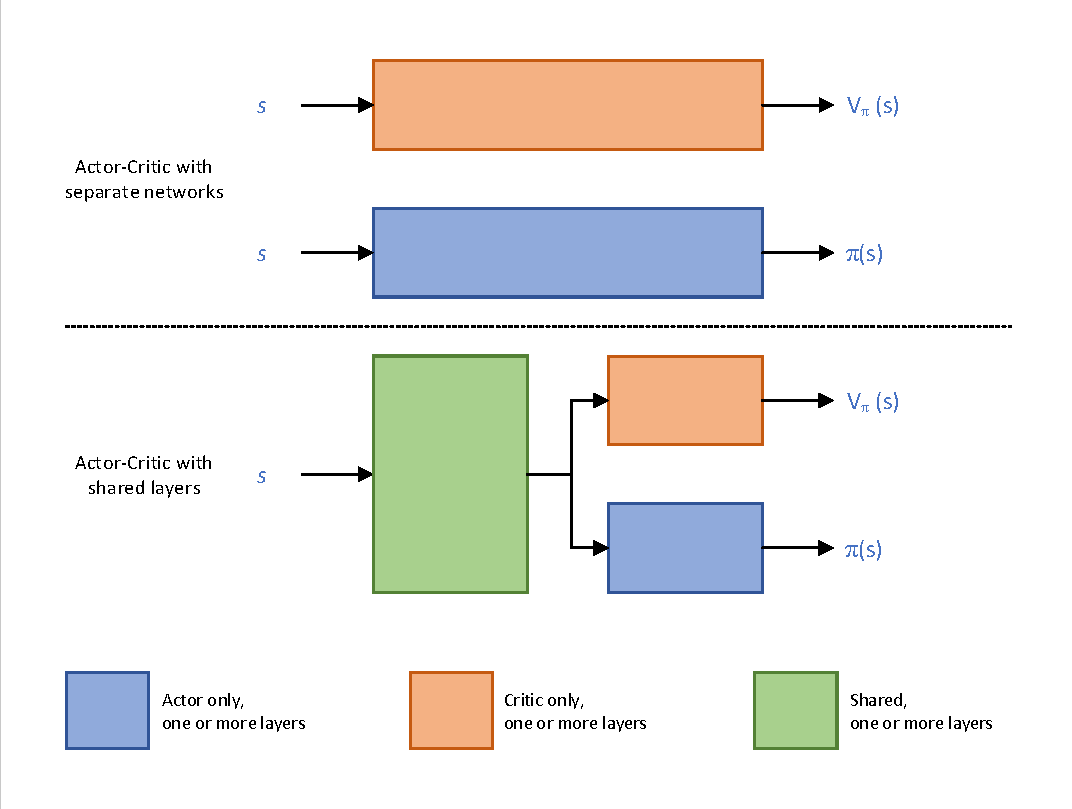
\includegraphics[clip, trim=10px 10px 10px 10px, width=0.85\columnwidth]{figures/rl/Actor_Critic_Architecture.pdf}
  \end{center}
  
  %\vspace*{-6pt}
  \caption[Actor-Critic Network Architectures]{Network architecture variants for actor-critic algorithms. The networks might be separate or with shared layers. (Adapted from \cite{foundations2019graesser})}
  \label{fig:actor_critic_architecture}
  %\vspace*{-12pt}
\end{figure}

We illustrated an example for the actor-critic network architecture in Figure \ref{fig:actor_critic_architecture}. While we could build the actor and the critic separately with two different networks, they will usually be constructed with a single network with separated network heads. The network then shares a certain amount of layers which learn basic feature representations. For example if we are dealing with images as input and are using a CNN to process them, the convolutional layers should be shared between the actor and the critic. This improves efficiency as we do not need to learn the feature representation twice. Since both the actor and the critic are propagating their error through the upper layers, they can be trained faster and unstable learning is reduced. After the shared layers, the actor and the critic have their own dedicated network output, which can consist out of a single layer or can be a complex network on its own. 

\begin{algorithm}[ht]
  \KwData{Actor learning rate $\alpha_A$, Critic Learning Rate $\alpha_C$ Entropy coefficient $\beta$}
  \KwResult{Optimized parameters for the actor $\theta_A$ and critic $\theta_C$}
  Initialize all the weights $\theta$ randomly \;
  \ForEach{episode}  {
   Sample trajectory $\tau = ((s_0, a_0, r_0), \dots, (s_T, a_T, r_T))$ with $\pi_\theta$ from the environment \;
    \For{$t=0, \dots, T$}  {
      $R_t(\tau) = \sum^T_{t'=t} \gamma^{t'-t}r_t$ \;
      Calculate $V_{\theta_C}(s_t)$ using the value network \;
      Calculate Entropy $H_t = - \sum_a \pi_{\theta_A}(a|s_t) \log \pi_{\theta_A}(a|s_t)$
    }
    \tcc{Calculate loss}
    $\mathcal{L}_{val}(\theta_C) = \frac{1}{T} \sum^T_{t=0}(V_{\theta_C}(s_t) - R_t(\tau))^2$ \tcp*{Value loss using MSE}

    $\mathcal{L}_{pol}(\theta_A) = \frac{1}{T} \sum^T_{t=0}\left(\left(V_{\theta_C}(s_t)-R_t(\tau)\right) \log \pi_{\theta_A}(a_t|s_t) - \beta H_t\right)$ \tcp*{Policy loss}

    \tcc{Update parameters with SGD optimizer}
    $\theta_C \leftarrow \theta_C - \alpha_C \nabla_{\theta_C} \mathcal{L}_{val}(\theta_C)$ \tcp*{Update Critic}
  
    $\theta_A \leftarrow \theta_A - \alpha_A \nabla_{\theta_A} \mathcal{L}_{pol}(\theta_A)$ \tcp*{Update Actor}

  }

  \caption[The Vanilla Actor-Critic Algorithm]{The vanilla actor-critic algorithm with entropy regularization.}\label{alg:ActorCritic}
 \end{algorithm}

The vanilla actor-critic method can be trained in a similar fashion as we did with REINFORCE and is shown in Algorithm \ref{alg:ActorCritic}. We changed a few things from REINFORCE, so lets quickly go through them:
\begin{itemize}
  \item We changed our notion for the application of the gradients. While we directly collected the gradients in Algorithm \ref{alg:REINFORCE}, we now calculate a loss. This makes it easier to add additional goals to the optimization (e.g. entropy). The loss is later converted into a gradient and applied by the SGD optimizer. Because we are now dealing with loss and the goal is to minimize the loss we have to change sign. By minimizing the loss we are performing gradient ascent on our objective function.
  \item We introduce integrated exploration and regularization with the addition of the entropy $H$ to the loss as we discussed in Section \ref{ssec:ImprovingPG}. The entropy is added to the loss for the actor and can be scaled with a new hyperparameter $\beta$.
  \item We are still using a for-loop over episodes, but it is possible to substitute this loop with a loop over an arbitrary number of individual steps (see Algorithm \ref{alg:PPO}).   
\end{itemize}

\paragraph{Estimating Advantage.}
The vanilla actor-critic algorithm is usually not used on its own. Instead a first extension is used: The \textit{Advantage Actor-Critic} (A2C) algorithm. When we talked about DQN Extensions in Section \ref{ssec:DQNExtensions} we briefly mentioned the advantage function $A(s, a)$. The advantage is a measure of how good an action is compared to all other actions. For DQN we compared the action only to other actions given that we know the optimal policy. This resulted in a maximal advantage of zero for the best action and a negative advantage for all other actions. This time we are instead looking at $A_\pi(s, a) = Q_\pi(s, a) - V_\pi(s)$. This is the advantage which measures the change in return if we take action $a$ and then always act according to our current policy. In other words, the advantage provides us with a relative measure of how good an action is compared to the average action our policy would choose. Before we look at how to estimate the advantage, let us first discuss why we should even care about advantage. Why do we need advantage when we have state-values?

Remember that we are currently training our policy by computing gradients based on the return we get by following the current policy in the environment. Our goal is to reinforce good actions and discourage bad actions. Since we compute our gradients from the return, we need the return to be negative for bad and positive for good actions to actually compute gradients which reflect reinforcement or discouragement of actions. Unfortunately this is not what usually happens: Many environments do not provide negative but only positive reward. So all actions are actually reinforced. To change this we need a relative measure which tells us how good an action is compared tp all other actions and this is exactly what the advantage function does. 

To compute the advantage we need two things: $V_\pi(s)$ and $Q_\pi(s, a)$. Currently our network only computes the value function, so should we further extend it to also compute the Q-Values? While this would be possible, it actually adds overhead into the network and Q-Values are harder to estimate than state-values, since Q-Value functions are more complex. Also learning Q-Values in continuous environments produces additional problems. So instead we want to estimate the Q-Values from the already estimated state-values. If we assume, that our estimate $V_\pi(s)$ is sufficiently accurate, we can estimate the Q-Value by:

\begin{align*}
Q_\pi(s_t, a_t) &= E_{\tau\sim\pi}\left[r_t + \gamma r_{t+1} + \gamma^2 r_{t+2} \dots + \gamma^n r_{t+n}\right] + \gamma^{n+1}V^*(s_{t+n+1}) \\
&\approx r_t + \gamma r_{t+1} + \gamma^2 r_{t+2} \dots + \gamma^n r_{t+n} + \gamma^{n+1}V_\pi(s_{t+n+1}) \\[15pt]
A_\pi(s_t, a_t) &= Q_\pi(s_t, a_t) - V_\pi(s_t) \\
&\approx r_t + \gamma r_{t+1} + \gamma^2 r_{t+2} \dots + \gamma^n r_{t+n} + \gamma^{n+1}V_\pi(s_{t+n+1}) - V_\pi(s_t)
\end{align*}

Using this $n$-step unrolling technique, we can estimate the Q-value with $n$ as a tradeoff parameter between variance and bias. Using more steps reduces bias, since $V_\pi(s)$ may be inaccurate, but at the same time it induces variance, since all rewards are sampled from a single trajectory. The idea is that variance increases the further we look into the future starting at step $t$ while the bias decreases. This means we are combining both to get the best result. Unfortunately deciding for an $n$ is not an easy choice and would require careful tuning. Therefore unrolling is done with a similar technique called \textit{Generalized Advantage Estimation} (GAE) which was proposed by Schulman et al. in 2015 \cite{schulman2015high}. Instead of using a fixed $n$ we instead compute the advantage using a weighted average over $n$-step advantages with $n = 1, 2, 3, \dots, k$. This technique further reduces the influence of variance and bias, while also making the choice of a hyperparameter easier. GAE can be written as:

\begin{align*}
  A_\pi(s_t, a_t) &= \sum^\infty_{l=0} (\gamma\lambda)^l \delta_{t+l} \\
  &\text{with } \delta_t = r_t + \gamma V_\pi(s_{t + 1}) - V_\pi(s_t) 
\end{align*}

While GAE still introduces a new hyperparameter in the form of $\lambda$ which controls how much we weight estimated advantages with further unrolling, this parameter does not introduce a hard boundary and therefore is much easier to tune. 

\begin{algorithm}[ht]
  \KwData{Actor learning rate $\alpha_A$, Critic Learning Rate $\alpha_C$ Entropy coefficient $\beta$}
  \KwResult{Optimized parameters for the actor $\theta_A$ and critic $\theta_C$}
  Initialize all the weights $\theta$ randomly \;
  \ForEach{episode}  {
   Sample trajectory $\tau = ((s_0, a_0, r_0), \dots, (s_T, a_T, r_T))$ with $\pi_\theta$ from the environment \;
    \For{$t=0, \dots, T$}  {
      Calculate $V_{\theta_C}(s_t)$ using the value network \;
      Calculate the advantage $A_\pi(s_t, a_t)$ using GAE. \;
      Calculate $V_{tar}(s_t)$ using the advantage. \;
      Calculate Entropy $H_t = - \sum_a \pi_{\theta_A}(a|s_t) \log \pi_{\theta_A}(a|s_t)$ \;
    }
    \tcc{Calculate loss}
    $\mathcal{L}_{val}(\theta_C) = \frac{1}{T} \sum^T_{t=0}(V_{\theta_C}(s_t) - V_{tar}(s_t))^2$ \tcp*{Value loss using MSE}

    $\mathcal{L}_{pol}(\theta_A) = \frac{1}{T} \sum^T_{t=0}\left(-A_\pi(s_t, a_t) \log \pi_{\theta_A}(a_t|s_t) - \beta H_t\right)$ \tcp*{Policy loss}

    \tcc{Update parameters with SGD optimizer}
    $\theta_C \leftarrow \theta_C - \alpha_C \nabla_{\theta_C} \mathcal{L}_{val}(\theta_C)$ \tcp*{Update Critic}
  
    $\theta_A \leftarrow \theta_A - \alpha_A \nabla_{\theta_A} \mathcal{L}_{pol}(\theta_A)$ \tcp*{Update Actor}

  }

  \caption[The Advantage Actor-Critic Algorithm]{The Advantage Actor-Critic (A2C) algorithm with entropy regularization.}\label{alg:A2C}
 \end{algorithm}

Algorithm \ref{alg:A2C} shows an updated version of the original actor-critic algorithm with GAE. Note that in praxis $V_{tar}$ is often calculated as $V_{tar} = A_{GAE}(s_t, a_t) + V_\pi(s_t)$ when using advantage estimation to avoid additional computation. 

\paragraph{Parallel environment interactions.}
We already developed techniques to solve most of the problems shown in Section \ref{ssec:ImprovingPG}, but there is still one remaining problem: Sample correlation. Since we cannot introduce a replay buffer - we are dealing with an on-policy algorithm - we have to generate a lot of training data to reduce sample correlation and variance before each update. Sampling all that data from a single environment running in a single process takes a lot of time and since episodes may be significantly dependent on the random initial state, we would need the agent to play through several whole episodes to gather good training data. In 2016 Mnih et al. showed, that it is possible to train an A2C agent in parallel on multiple environments with their \textit{Asynchronous Advantage Actor-Critic} (A3C) algorithm \cite{mnih2016asynchronous}.

When training the agent in parallel on multiple environments we want to create multiple copies of the same environment (and our agent) which gather trajectories independent of each other. Further, we want to initialize them with a different random seed to generate different trajectories due to randomness in environment transitions or agent action choices. The workers then continuously gather the training data from agent-environment interactions. This data will be used to calculate updates for a global network, which will then be pushed back to the workers periodically. This procedure can be done in two different ways: Synchronous and Asynchronous. Though A3C only uses asynchronous parallelization we will also briefly discuss synchronous parallelization as well.
\begin{itemize}
  \item \textbf{Synchronous Parallelization.} In synchronous parallelization all workers are working with the same copy of the network. Workers will gather a trajectories of a certain length and then wait for all other workers to finish. The trajectories are then combined and used to update the global network. After the global network has updated, each worker pulls the updated parameters to its own network copy and then continuous to collecting new trajectories. This type of parallelization is often used for A2C. The use of dedicated network copies can be avoided, if training is only done on a single machine.
  \item \textbf{Asynchronous Parallelization.} In asynchronous parallelization workers also collect trajectories, but they additionally compute the gradients and then directly push the gradients to the global network. The workers do not wait for each other and thus may work with a slightly outdated network copy. 
\end{itemize}
Both parallelization methods have their pros and cons. While synchronous parallelization works well on a single machine, the waiting mechanism may significantly slow down a distributed training processes. On the other hand for non-blocking asynchronous parallelization, the computation of gradients on slightly outdated network copies makes training less stable. Nevertheless, both methods work well and vastly reduce the impact of sample correlation and variance for on-policy PG methods. 


\subsection{Proximal Policy Optimization} \label{ssec:PPO}
The A2C algorithm addresses every problem we talked about in Section \ref{ssec:ImprovingPG}. Still if we look at the learning curve in in Figure \ref{fig:a2c_cartpole} which shows the training progress on the simple environment CartPole, we can see that learning tends to still be unstable and even suffers from \textit{performance collapse}. How is that possible? To understand the origin of this problem, we need to look back at our basic procedure of how we are improving our policy using policy gradients.

\begin{figure}[ht]
  
  \begin{center}
      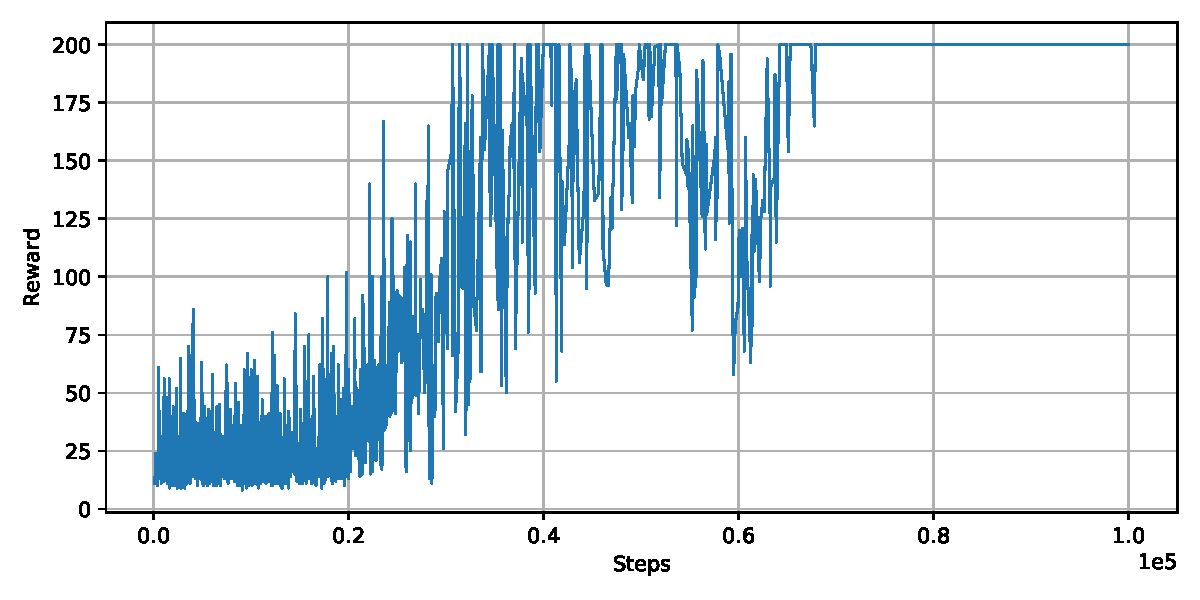
\includegraphics[clip, width=0.8\columnwidth]{figures/rl/a2c_cart_pole_plot.pdf}
  \end{center}
  
  %\vspace*{-6pt}
  \caption[Learning Curve for A2C on CartPole]{Reward per episode for an agent trained with the A2C algorithm on the CartPole environment over $100k$ training steps (roughly 600 episodes). Notice the brief performance collapse around 600k training steps.}
  \label{fig:a2c_cartpole}
  %\vspace*{-12pt}
\end{figure}

In PG algorithms, we use a policy $\pi_\theta$ which is parameterized by the weights of our neural network. This policy is used to generate a trajectory in our environment from which we compute the policy gradient $\nabla_\theta J(\pi_\theta)$. During optimization we therefore generate a sequence of policies $\pi_1, \pi_2, \dots, \pi_n$ from the the policy space $\Pi$ (the set of all policies). The problem is we are not actually directly searching for a policy in that space. Instead we are searching the policy in the parameter space $\Theta = \{\theta \in \mathbb{R}^m\}$ with $m$ being the number of parameters in our network. Unfortunately distances in policy space and in parameter space are not the same with respect to $\theta$. If we take two pairs of parameters $(\theta_1, \theta_2)$ and $(\theta_2, \theta_3)$ with the same distance in the parameter space, their mapped policies in policy space might not have the same distance:

\[d(\theta_1, \theta_2) = d(\theta_2, \theta_3) \cancel{\Leftrightarrow} d(\pi_{\theta_1}, \pi_{\theta_2}) = d(\pi_{\theta_2}, \pi_{\theta_3}) \]

The hypersurface on which we are performing our gradient ascent is not equal to the hypersurface we actually care about. This produces a semantic gap in our training process. Simply adjusting the learning rate $\alpha$ to a small value does not simply fix this problem. A small learning rate will only slow down learning and raise the probability of getting stuck in a local maximum. On the other hand we cannot accept occasional learning collapses, since learning collapses mean that we will immediately and dramatically reduce the quality of our training data. Recovering from a performance collapse can therefore take a long time. So how can we prevent them, while still learning in parameter space? The answer to this are \textit{trust regions}. The idea is to estimate the change in policy space. We then define a maximal distance "around" our old policy in policy space - called trust region - which is the maximum distance the new policy is allowed to deviate from the old policy. Moreover we want to guarantee, that the performance of the new policy is always better than the performance of the old policy.

In 2015 Schulman et al. were able to provide mathematical foundations with made the computation of trust regions and \textit{guaranteed monotonic improvement} of the policy possible. They also proposed an algorithm called \textit{Trust Region Policy Optimization} (TRPO) \cite{schulman2015trust}. Unfortunately even though their algorithm works, it is hard to implement and computationally very expensive, since it relies on second order derivates. To overcome these problems, they extended their work in 2017, proposing a simplified algorithm called \textit{Proximal Policy Optimization} (PPO) which even outperforms their pervious one in many environments \cite{schulman2017proximal}. PPO is computationally as expensive as vanilla actor-critic variants and thus PPO is one of the most used reinforcement learning algorithms today. In the remainder of this Section, we want to take a look at how PPO achieves its goal of monotonic policy improvement, while staying computationally inexpensive.

\paragraph{Monotonic Improvement.}
Instead of trying to directly maximize the expected return $J(\pi)$, we can instead maximize a different objective. To achieve monotonic improvement, we formulate a new objective based on the \textit{relative policy performance identity}. If we have some policy $\pi$ and update that policy to get $\pi'$, we define their relative policy performance identity as

\begin{equation} \label{eq:MonotonicImprovement}
  J(\pi') - J(\pi) = E_{\tau \sim \pi'}\left[\sum_{t\geq0} A_\pi(s_t, a_t)\right]
\end{equation}

which is their difference in expected return. With this objective our optimization problem becomes $\max_\pi' (J(\pi') - J(\pi))$ which ensures, that $J(\pi') - J(\pi) \geq 0$. The worst case is simply not changing the policy, such that $\pi'=\pi$.

The problem with Equation \ref{eq:MonotonicImprovement} is that it uses an expectation over a trajectory sampled from $\pi'$ - which we obviously do not have access to at that point. We therefore need a way to estimate trajectories from $\pi'$. If we assume that two successive policies $\pi$ and $\pi'$ are relatively close, we can also assume that the resulting state distributions we observe when interacting with the environment are also similar. Therefore we can use a method known as \textit{importance sampling} which estimates an unknown distribution from data sampled from a known distribution. This is done by computing weights which increase rewards which are more likely under $\pi'$ and decrease rewards which are less likely. These weights are calculated by the ratio of action probabilities between $\pi$ and $\pi'$: $\frac{\pi'(a_t, s_t)}{\pi(a_t, s_t)}$. We then can estimate the relative policy performance identity by

\begin{equation}
  J(\pi') - J(\pi) = E_{\tau \sim \pi}\left[\sum_{t\geq0} A_\pi(s_t, a_t) \frac{\pi'(a_t, s_t)}{\pi(a_t, s_t)}\right] = J^{CPI}_\pi(\pi')
\end{equation}

thus being only dependent on samples generated by the current policy. The new objective called the \textit{conservative policy iteration} (CPI) $J^{CPI}_\pi(\pi')$  is also called the \textit{surrogate objective}, since it indirectly optimizes the original objective. It can be proven that the gradient with respect to $\theta$ of the surrogate objective is equal to the gradient of the original objective. We omit the proof here, but it can be found in \cite{foundations2019graesser}. 

If the gradient of the original and the surrogate objective is the same, one could ask the question why we even need the new objective. Also we only approximate $J(\pi') - J(\pi)$, so how do we guarantee that $J(\pi') - J(\pi) \geq 0$? The reason behind our new objective is that it allows us to bound the error. Achim et al. \cite{achiam2017constrained} showed that using the Kullback-Leibler (KL) divergence between two successive policies, we can bound the error to

\[|(J(\pi') - J(\pi)) - J^{CPI}_\pi(\pi')| \leq C \cdot \sqrt{E_t\left[KL\left(\pi'(a_t, s_t)||\pi(a_t, s_t)\right)\right]}\]

From this, we can easily derive a form which allows us to determine if $J(\pi') - J(\pi) \geq 0$:

\begin{equation} \label{eq:MonotonicImprovement2}
  J(\pi') - J(\pi) \geq J^{CPI}_\pi(\pi') - C \cdot \sqrt{E_t\left[KL\left(\pi'(a_t, s_t)||\pi(a_t, s_t)\right)\right]}
\end{equation}

Looking at Equation \ref{eq:MonotonicImprovement2} we can see, that $J(\pi') - J(\pi) \geq 0$ only holds, if $J^{CPI}_\pi(\pi')$ is greater than the maximum error. If we only update our policy if this condition holds, we can guarantee policy improvement even if we only estimated  $J(\pi') - J(\pi)$. In a worst case scenario the best new policy will be the old policy, since if $J^{CPI}_\pi(\pi') = 0$ and $KL(\pi||\pi) = 0$ we can still accept the old policy as new policy. Using Equation \ref{eq:MonotonicImprovement2} we can finally formulate an updated version of the optimization problem:

\[\argmax_{\pi'}(J^{CPI}_\pi(\pi') - C \cdot \sqrt{E_t\left[KL\left(\pi'(a_t, s_t)||\pi(a_t, s_t)\right)\right])}\]

The remaining question now is how to implement this optimization problem in practice. Usually the error term is directly bounded to some constant $\delta$ which directly limits how large the KL divergence can be:

\[E_t[KL(\pi_\theta(a_t|s_t)||\pi_{\theta_{old}}(a_t|s_t))] \leq \delta\]

Of course $\delta$ is a hyperparameter that must be tuned for each individual RL problem. Since we are usually learning from a single step (or a small batch), our expectation is also written as an expectation over a single step. Since we are maximizing our objective in parameter space we are now writing our equation as dependent on these parameters $\theta$, with $\pi' = \pi_\theta$ and $\pi = \pi_{\theta_{old}}$. Therefore we arrive at the final surrogate objective:

\begin{align*}
  &\max_\theta E_t\left[\frac{\pi_\theta(a_t|s_t)}{\pi_{\theta_{old}}(a_t|s_t)}A_{t,\pi_{\theta_{old}}} \right] \\
  &\text{subject to } E_t[KL(\pi_\theta(a_t|s_t)||\pi_{\theta_{old}}(a_t|s_t))] \leq \delta
\end{align*}

With this surrogate objective we are now maximizing a linear approximation of $J(\pi') - J(\pi)$ with an imposed trust region, limiting the difference between the old and the new policy and thus avoiding performance collapse. Our new objective also now guarantees monotonic improvement.

\paragraph{The PPO Algorithm.}
The \textit{Proximal Policy Optimization} (PPO) algorithm was proposed by Schulman et al. in 2017 \cite{schulman2017proximal}. It uses the idea of trust regions with a minimum of additional computation. It also replaces the hyperparameter $\delta$ with a new hyperparameter which is easier to tune. In their original paper Schulman et al. proposed two different variants for the trust region constraint: An adaptive KL penalty - which uses a variable $\delta$ - and a clipped objective. In their tests, both variants proved to have good performance, but since the clipped objective is easier to tune, easier to implement and at least as good as the version with the KL penalty we will omit further details on adaptive KL penalty. 

To simplify our equations and add a little more clarity we will only write $A_t$ for $A_{t, \pi_{\theta_{old}}}$ in the following. We also define our probability ratio as $r_t(\theta) = \frac{\pi_\theta(a_t|s_t)}{\pi_{\theta_{old}}(a_t|s_t)}$. This way we can rewrite our surrogate objective as

  \[J^{CPI}(\theta) = E_t\left[\frac{\pi_\theta(a_t|s_t)}{\pi_{\theta_{old}}(a_t|s_t)}A_{t, \pi_{\theta_{old}}}\right] = E_t[r_t(\theta)A_t]\]

We will now take a look at the \textit{clipped surrogate objective}, which adds a clipping term to $J^{CPI}$:

\[J^{CLIP}(\theta) = E_t[\min(r_t(\theta)A_t, clip(r_t(\theta), 1-\epsilon, 1+\epsilon)A_t)]\]

The interesting thing is, that we can use this objective without adding a constraint for the KL divergence. The reason behind this can be explained by looking at the possible ways to maximize $J^{CPI}$. If we look at one step of training and some $A_t > 0$ one option to maximize $J^{CPI}$ would be to just perform a large policy update - thus maximizing $r_t(\theta)$. This is not what we want, because we already know that we are optimizing in parameter space and large policy updates are risky. In $J^{CLIP}$ we therefore clip the value of $r_t(\theta)$ to an $\epsilon$-neighborhood between $(1-\epsilon)A_t$ and $(1+\epsilon)A_t$. As long as $r_t(\theta)$ is in the interval $[1-\epsilon, 1+\epsilon]$, $J^{CLIP}$ is equal to $J^{CPI}$, but as soon as the new action probability diverges too much from the old policy the value is clipped. Hence, policy updates under the clipped objective function are always safe and we do not need an additional constraint.

\begin{algorithm}[h!]
  \KwData{Actor learning rate $\alpha_A$, Critic Learning Rate $\alpha_C$ Entropy coefficient $\beta \geq 0$, Clipping variable $\epsilon \geq 0$, Number of Epochs $K$, Number of Actors $N$, Time Horizon $T$}
  \KwResult{Optimized parameters for the actor $\theta_A$ and critic $\theta_C$}
  $M \leftarrow NT$ \;
  Initialize all the weights $\theta$ randomly \;
  Initialize the old actor network $\theta_{A_{old}}$ \;
  \For{$i=1, 2, \dots$}  {
    $\theta_{A_{old}} \leftarrow \theta_A$ \;
    \For{$actor = 1, 2, \dots, N$}{
      Sample trajectory $\tau = ((s_0, a_0, r_0), \dots, (s_T, a_T, r_T))$ from the environment with policy using $\theta_{A_{old}}$. \;
      Calculate $V_{\theta_C}(s_0), \dots V_{\theta_C}(s_T)$ using the value network \;
      Compute advantages $A_0, \dots, A_T$ using $\theta_{A_{old}}$ \;
      Calculate $V_{tar}(s_0), \dots V_{tar}(s_T)$ using the advantage and the value network $\theta_C$. \;
    }
    Construct a \textit{batch} with size $M$ from trajectories, advantages and target V-values. \;

    \For{$epoch=1, 2, \dots, K$}{
      \ForEach{minibatch $m$ in \textit{batch}}{
        \tcc{The following are computed over the whole batch}
        Calculate $r_m(\theta_A)$ \;
        Calculate $J^{CLIP}_m(\theta_A)$ using advantages $A_m$ and $r_m(\theta_A)$ \;
        Calculate entropies $H_m$ using actor network $\theta_A$ \;
        
        \tcc{Calculate loss}
        $\mathcal{L}_{val}(\theta_C) = \frac{1}{M} \sum^M_{t=0}(V_{\theta_C}(s_t) - V_{tar}(s_t))^2$ \tcp*{Value loss using MSE}
    
        $\mathcal{L}_{pol}(\theta_A) = \frac{1}{M} \sum^M_{t=0}\left(J^{CLIP}_t(\theta_A) - \beta H_t\right)$ \tcp*{Policy loss}

        \tcc{Update parameters with SGD optimizer}
        $\theta_C \leftarrow \theta_C - \alpha_C \nabla_{\theta_C} \mathcal{L}_{val}(\theta_C)$ \tcp*{Update Critic}
      
        $\theta_A \leftarrow \theta_A - \alpha_A \nabla_{\theta_A} \mathcal{L}_{pol}(\theta_A)$ \tcp*{Update Actor}

      }

    }

  }

  \caption[The PPO Algorithm with Clipped Surrogate Objective]{The PPO algorithm with clipped surrogate objective as an extension to synchronous parallelized A2C. (Adapted from \cite{foundations2019graesser}.)}\label{alg:PPO}
 \end{algorithm}


Removing the KL divergence constraint makes the clipped objective function computationally inexpensive. The only computations that are done are the probability ratio $r_t(\theta)$ and the advantage $A_t$. Both of them are the minimal computational cost we have to invest for any policy update. Algorithm \ref{alg:PPO} shows PPO with a clipped objective function as an extension of the actor-critic algorithm from Section \ref{ssec:A2C}. We also use synchronous parallelization.

 The algorithm shown has some major differences with the original A2C algorithm from Algorithm \ref{alg:A2C} so lets go over them:
\begin{itemize}
  \item We got a few new hyperparameters. The number of actors defines the number of parallel agents. We will talk about the number of epochs and the time horizon later on.
  \item \textit{Line 4}: Our Main loop changed from episodes to an infinite loop. Usually this outer loop will train for a fixed number of steps.
  \item \textit{Lines 6-11}: Each actor trains for a set amount of steps in its own copy of the environment. We call this amount of steps the \textit{Time Horizon} $T$. Since we are using the synchronous variant of A2C, each actor uses the same network weights. After sampling the trajectory we are computing state values and estimating advantages via GAE for each step. We are also computing the V-target values.
  \item \textit{Lines 12-14}: After we have generated the trajectories and computed state-values and advantages, we create a batch for the network updates. Since the objective function only needs samples from the old policy $\pi_{\theta_{old}}$, we can use data from the trajectory multiple times. This increases sample efficiency. We create random samples from of our batch of training data with size $T$. These smaller batches are called \textit{minibatches} and we compute a parameter update for each of them. We will repeat this for $K$ epochs.
  \item \textit{Lines 15-21}: We calculate the probability ratio $r_m(\theta_A)$ our objective $J^{CLIP}_m(\theta_A)$ and the entropy $H_m$ based on the current minibatch. We then calculate the loss for the actor and the critic and apply the resulting gradients with the SGD optimizer of choice. 
\end{itemize}

\subsection{Alternative Actor-Critic Algorithms} \label{ssec:AlternativeCombinedMethods}
We already presented one of the most well-known members of the actor-critic family - the PPO algorithm - in Section \ref{ssec:PPO}. In this section we want to give a short introduction into two additional members of the actor-critic family: ACER which aims at improving sample-efficiency by making it possible to learn from past experiences and ACKTR, which proposes an alternative trust region algorithm. 

\paragraph{ACER.}
\textit{Actor-Critic with Experience Replay} (ACER) was developed in 2016 by Wang et al. \cite{wang2016sample}. The goal of ACER was to create an actor-critic successor which could handle off-policy training and thus being more sample efficient. ACER also implements trust-region policy optimization. \\
At its base, ACER changes the actor-critic architecture to learn Q-Values instead of V-Values. They do this, by using the Retrace algorithm by Munos et al. \cite{munos2016safe} which estimates target Q-Values with minimal bias and variance and has been proven to converge:

\begin{align*}
  &Q^{ret}(s_t, a_t) = r_t + \gamma \bar{r}_{t+1}(\theta) \left[Q^{ret}(s_{t+1}, a_{t+1}) - Q_\pi(s_{t+1}, a_{t+1})\right] + \gamma V_\pi(s_{t+1}) \\
  &\text{with } \bar{r}_t(\theta) = \min(c, r_t(\theta))
\end{align*}

After sampling a trajectory we can compute the values for $Q^{ret}$ from the last timestep backwards, since $Q^{ret}(s_T, a_T) = 0$. We can then use $Q^{ret}$ as target value and compute the mean square error loss for backpropagation. \\
For the training of the actor, ACER also uses the target Q-Values. Similar to PPO, sample returns will be weighted by the probability ratio between the old and the new policy $r_t(\theta)$. To achieve this, we need to save the probability distribution from our policy in our trajectory. The problem for off-policy training is that the importance weights may become very large causing training instability. This is prevented by clipping the importance weights to a fixed value $c$. To ensure an unbiased estimation they also add a correction term which they call the \textit{truncation with bias correction trick} 

\begin{align*}
  \mathcal{L}^{acer}_{pol}(\theta_A) = &\bar{r}_t(\theta) \log \pi_A(a_t|s_t)[Q^{ret}(s_t, a_t) - V_{\theta_C}(s_t)] \\ 
  &+ E_{a\sim\pi} \left(\left[\frac{r_t(\theta, a) - c}{r_t(\theta, a)}\right]_{+} \log \pi_{\theta_A}(a|s_t)[Q_{\theta_C}(s_t, a) - V_{\theta_C}(s_t)] \right)
\end{align*}

\begin{align*}
  &\text{with } r_t(\theta, a) = \frac{\pi_\theta(a|s_t)}{\pi_{\theta_{old}}(a|s_t)} \\
  &\text{and } [x]_+ = 
  \begin{cases} 
    x, & \text{if}\ x > 0 \\
    0, & \text{otherwise}
  \end{cases}  
\end{align*}
 

The above expression also uses a baseline $V_{\theta_C}(s_t)$ which is subtracted to reduce variance. The first term is the standard loss, weighted by our clipped importance weights and the second term is the correction term. \\
We already saw that actor-critic variants may have problems when updating the policy, since updates take place in the parameter space. Similar to PPO, ACER uses a trust region when performing updates. However ACER uses a different method: Instead of constraining the policy to not deviate too much from its predecessor, ACER maintains an \textit{average policy network}. This network represents a running average of past policy networks. When updating, ACER computes the KL divergence between the new and the average policy network and thus bounds the policy from deviating too far.

\paragraph{ACKTR.} \textit{Actor Critic using Kronecker-Factored Trust Region} (ACKTR) has been developed in 2017 by Wu et al. \cite{wu2017scalable}. ACKTR combines an improved optimization method called \textit{natural gradient descent} with yet another idea of how to compute trust regions for actor-critic updates. ACKTR has proven to have higher sample efficiency and learn better results in less time than A2C or TRPO. \\
Today most RL algorithms use stochastic gradient descent to calculate gradients for the network. SGD optimizers use first order derivates on the loss function meaning they compute the slope of the loss function at a given point. First oder derivates are fast and easy to compute and combined with extensions like momentum provide reasonably fast results. However SGD has to face a similar problem we explored earlier: Changes to the weights are computed by choosing  the largest change for the objective at the current point in parameter space assuming an equal change to the objective (policy space). We also do not look at the second derivate, which makes SGD very sensitive to the learning rate, because a large descent at a point in some direction does not mean we can go in that direction forever and still improve. We saw, that it is possible to limit the change in policy space by setting an upper bound for the KL divergence - ensuring our new policy would be "close enough" to the old policy. But what if we were able to optimize our policy in policy space? This would not only solve the problem of diverging from the optimum, but also speed up learning, as our gradient descent would converge faster if each step would be guided directly to the optimum. \\
In 1998, Shun-Ichi Amari presented his approach of using a \textit{natural gradient} instead of standard SGD \cite{amari1998natural}. The idea is that we build a connection between each parameter from our model (from parameter space) to the policy space which tells us how great of an impact the change of each parameter will have in policy space. This way we can compute the natural gradient as the largest change in objective per unit change in our model parameters. By performing these weighted gradient descent steps in parameter space which the resulting changes in policy space will have the same distance.
If we look at gradient descent and some loss $\mathcal{L}(\theta)$, the steepest descent direction can be defined as the vector $d$ which minimizes $\mathcal{L}(\theta + d)$ under the constrained that the squared length of $|d|^2 \leq \epsilon$. This length of $d$ is $\sum_i (d_i)^2$ in an euclidean space and $\sum_{i, j} g_{i, j}d_i d_j$ in any arbitrary coordinate system. The values $g_{i, j}$ are given by a positive semi-definite matrix $G$. The second formula for the distance is equal to the first one if $G$ is the identity matrix $I$ (which is true for any euclidean space). Amari showed, that we can define the direction of the steepest gradient descent in any space as 
\[\tilde{\nabla}\mathcal{L}(\theta) = G^{-1}\nabla\mathcal{L}(\theta) \]. 
So how do we compute the matrix $G$? Amari showed, that it is possible to calculate $G$ by using the the \textit{Fisher Information Matrix} (FIM), which is given by 

\begin{align*}
  F &= E_{p(x|\theta)} \left[\nabla \log p(x|\theta) \nabla \log p(x|\theta)^T\right] \\
  &\approx \frac{1}{N} \sum^N_{i=1} \nabla \log p(x_i|\theta) \nabla \log p(x_i|\theta)^T
\end{align*}

for a distribution $p(x|\theta)$ which is generated by our model parameterized by $\theta$. The interesting property of the FIM is that it is equal to the Hessian (the second order derivate) of the KL-divergence. Therefore the FIM defines the local curvature in policy space. The natural gradient is therefore defined as:

\[\tilde{\nabla}_\theta\mathcal{L}(\theta) = F^{-1}\nabla_\theta\mathcal{L}(\theta)\]

The computation for natural gradient descent follows Algorithm \ref{alg:NaturalGradient} and is very similar to SGD with the exception of the computation of the FIM. 

\begin{algorithm}[h!]
  \KwData{Learning rate $\alpha$}
  \KwResult{Optimal parameters $\theta$ minimizing the loss function $\mathcal{L}(\theta)$}
  
  \While{Not Converged} {
    Compute the loss $\mathcal{L}(\theta)$ like before. \;
    Compute the gradient for the loss $\nabla_\theta \mathcal{L}(\theta)$ \;
    Compute the FIM from the trajectory. \;
    Compute the natural gradient $\tilde{\nabla}_\theta\mathcal{L}(\theta) \leftarrow F^{-1}\nabla_\theta\mathcal{L}(\theta)$ \;
    $\theta \leftarrow \theta - \alpha \tilde{\nabla}_\theta\mathcal{L}(\theta)$ \;
  }
  
  \caption[The Natural Gradient Descent Algorithm]{The Natural Gradient Descent Algorithm.}\label{alg:NaturalGradient}
 \end{algorithm}


Unfortunately even though the idea of natural policy gradient seems promising, and in 2002 Sham Kakade was able to show that the natural gradient can be applied to policy gradient methods and converges faster than optimization with SGD in an RL setting \cite{kakade2002natural}, the computation of the FIM is computationally very expensive. Even worse, for the size of nowadays neural networks with millions of parameters, the sheer size of the FIM would exceed main memory capacity. The only way we are able to use the FIM would be to find a reasonably good approximation. In 2015 James Martens and Roger Grosse presented their novel method called \textit{Kronecker-Factored Approximate Curvature} (KFAC) \cite{martens2015optimizing} which is specifically designed to efficiently approximate FIM matrices for neural networks. The idea is to calculate approximations for the FIM layer-wise by assuming, that second-order statistics of the activations in layer $l$ and the backpropagated derivates are uncorrelated. While this assumption is not exact, in reality it still yields good results. KFAC can be used to train both the actor and the critic if we define the output of the critic as a Gaussian distribution - for which we can then calculate the Fisher matrix. 
%Let $p(y|x)$ denote the output distribution of a neural network and $L = \log p(y|x)$ denote the log-likelihood. In the $l$th layer we have our weight matrix $W \in \mathbb{R}^{C_{out}\times C_{in}}$ where $C_{in}$ is the number of input neurons and $C_{out}$ is the number of neurons in the current layer. The current layer receives a vector $a \in \mathbb{R}^{C_{in}}$ from the $(l-1)$th layer and computes its output vector as a weighted sum $z = Wa$. Note that we did not apply the activation function yet. The weight gradient for our layer is then given by $\nabla_W L = (\nabla_sL)a^T$. We further define an operation $vec\{\}$ which vectorizes a matrix by stacking the columns on top of each other and denote the Kronecker product as $A \otimes B$ - which multiplies each element in matrix $A$ with matrix B such that $A \otimes B = (a_{i, j} B)$. We then can write the Fisher matrix for layer $l$ as 

%\begin{align*}
%  F_l &= E[vec\{\nabla_W L\}vec\{\nabla_W L\}^T] = E[aa^T \otimes \nabla_sL(\nabla_s L)^T \\
%  &\approx E[aa^T] \otimes E[\nabla_sL(\nabla_s L)^T]

%\end{align*}

Since we are only working on a approximation of the Fisher matrix and it was observed, that in the context of deep RL unbounded updates can lead to large policy updates, ACKTR also uses a trust region method. Ba et al. showed, that since the Fisher matrix has a direct connection to the KL-divergence, it can be used as a replacement when formulating the trust region \cite{ba2016distributed}. This can be done by setting the effective step size $\eta$ for an update of the parameters to 
\[\eta = \min\left(\eta_{max}, \sqrt{\frac{2\delta}{\mathbf{v}^T\hat{F}\mathbf{v}}}\right)\]

where $\delta$ is the trust region radius, $\mathbf{v} = \Delta\theta$ is a vector representing the parameter change and $\hat{F}$ is the Fisher matrix approximation.
ACKTR has shown exceptional good performance in comparison with A2C and TRPO in both maximum performance and wall-clock time.


\subsection{Learning with Curiosity} \label{ssec:Curiosity}
So far all our agents tried to maximize one thing: The total reward they get from the environment. This behavior produces multiple problems at once: 

\begin{itemize}
  \item The agents learned behavior is directly dependent on the reward function, so correctly shaping the reward is crucially improtant for every new environment.
  \item If rewards are only given in a very sparse setting, agents may fail completely at exploring the environment to the point where they actually get rewarded. This also happens because we learn from loss and our loss is only dependent on the reward we are getting. If our agent is not able to get any reward, it will be unable to learn anything.
  \item Even if the agent is able to learn, it fails at deeply exploring the environment further, because every change in policy results in less reward for the moment.
\end{itemize}

If we look at all these problems, they are all related to a problem of exploring the environment. In the past, we explored the environment by random chance, but that does not seem to be sufficient. As a human, how do we get motivated to do something? Do we only learn or explore if we get rewarded for it with something that is given to us? The answer is no - we get reward, but it is not given to us, it is intrinsic to ourselves: We are curious about our surroundings and by satisfying that curiosity we generate "reward". Curiosity drives us to learn things that do not serve any need at the moment, but may become handy sometimes in the future. This idea motivates to extend the basic reward function for our agent to include a term for curiosity.

Modeling curiosity for RL agents has been maily explored in two different approaches: Encouraging the agent to explore novel states  or encouraging the agent to perform actions which outcome cannot be predicted well. Measuring novelty has been shown to be difficult, since it requires to model the unknown statistical dirstribution of environmental states. In 2017 Pathak et al. proposed an \textit{Intrinsic Curiosity Module} (ICM) which generates inrinsic reward $r^i_t$ additinal to the extrinsic reward $r^e_t$ from the environment. They showed, that it is possible to train agents using purely intrinsic reward and that agents trained with both intrinsic and extrinsic reward, outperform agents trained purely with extrinsic reward.

Let us take a look at how the ICM works. The idea of the ICM is to use prediction error as an idicator for curiosity reward. Intuitively this makes sense, since prediction error can be seen as the agent being surprised by a state. But we have to be slightly more precise when it comes to this prediction error. Let us look at an example where the agent gets an observation from a camera. Under low light conditions the image will get more and more noisy, making situations with low light more interesting. Similar things are happening with various other things, like a TV outputting static noise, or leafs moving in the wind. In all these situations our observation (especially observations which are images) will change unpredictably and thus be surprising to the agent. We are therefore interested in a feature representation, which is only dependent on things the agent has influence over or which direcly influence our agent in the environment. Everything else is just noise and should be ignored. With all this information let us look at curiosity from a mathematical point of view. To calculate the reward we will use an embedding network which transforms the observation of the current state into a good representation $\phi(s)$. We will then use a \textit{forward dynamic network} which should predict the representation of the next state $\hat{\phi}(s_{t+1})$ from the current state and action the agent took in state $s_t$ so $p(\phi(s_{t+1})|s_t, a_t)$. For a given transition tuple $(s_t, a_t, s_{t+1})$ the intrinsic reward is therefore defined as $r_t = - \log p(\phi(s_{t+1})|s_t, a_t)$ and usually calculated using the mean square error:

\[r^i_t = \frac{\eta}{2}||\hat{\phi}(s_{t+1}) - \phi(s_{t+1})||^2\]

with a scaling factor $\eta > 0$. The prediction error for a state will naturally be higher if the state or very similar states have not been often explored in the past, thus encouraging the agent to do so in the future.   
Burda et al. investigated the performance of this intrinisic reward in combination with several feature spaces for forward dynamics \cite{burda2018large}. Two different approaches were found which both yield good results: 

\begin{enumerate}
  \item \textbf{Random Features (RF).} Random features are generated by a convolutional neural network. All parameters of that network will be fixed after the inital random initialization. This procedure results in stable features, but the features itself are not guaranteed to filter out any unnecessary information or contain all necessary ones. Surprisingly random features were still found to yield good results. Also random features are easy to implement and do not require extra training time.
  \item \textbf{Inverse Dynamics Features (IDF).} Inverse dynamics features were initally proposed for the ICM and are generated by another neural network. Given two states $s_t, s_{t+1}$ the network should predict the action $a_t$ the agent chose in state $s_t$. The networks first layers are used as a common neural network $\phi$ to embedd the observations. The idea is, that by training this network to predict the action, the needed feature representation will ignore all aspects of the observation which are not under the agents immediate control. However this representation will not show aspects of the environment which will influence the agent which are not under its direct control.
\end{enumerate}

While both approaches have shown to work well with the ICM, they both failed at reliably eliminating the influence of stochastic transitions in the environment. Even with IDF features, if the agent has the possibility to influence the appearance of stochastic features (like randomly changing static noise on a TV) it would tend to only explore these stochastic states after some time. Also when using IDF we are dealing with stochasticity induced by sampling an action from our policy which cannot be predicted by our deterministic predictor network. Burda et al. therefore proposed in another paper a new approach which they called \textit{Random Network Distillation} (RND) \cite{burda2018exploration}.

RND is not an embedding for the observation and instead replaces the whole ICM. The inrinsic reward is generated by a random prediction problem. This problem is build by two neural networks: The first network is called the \textit{target} network which is randomly initialized and fixed - similar to the random features network from before. This target network takes the observation and transforms it into a random feature representation $f : \mathcal{O} \rightarrow \mathbb{R}^k$. We then construct a second network with the same architecture called the \textit{predictor} network which also takes the observation as input $\hat{f} : \mathcal{O} \rightarrow \mathbb{R}^k$. The predictor network is trained to minimize the mean square error between its own output and the target network $||\hat{f}(s) - f(x)||^2$. The idea is, that the prediction error will be larger for observations which are dissimilar to observation seen in the past. It could be shown, that gradient descent is unable to mimic the target network perfectly for any input and therefore the error can be used to generate the intrinsic reward signal. The authors showed, that for actor-critic variants it can be beneficial to implement intrinsic reward with an additional value head for the network (one predicting the state value for expected environment reward and one for expected intrinisic reward). They showed that this method can improve learning further if rewards are not clipped at the end of an episode (restart is just the next state). 

Curiosity - especially with RND - has shown to vastly improve the performance of PPO especially for environments with sparse reward. It also has been proven to be beneficial for environments with dense reward - leading to agents which learn both faster and reach a higher final reward. Curiosity can be combined with any RL algorithm, but only has been extensively studied in combination with PPO so far.